% Options for packages loaded elsewhere
% Options for packages loaded elsewhere
\PassOptionsToPackage{unicode}{hyperref}
\PassOptionsToPackage{hyphens}{url}
\PassOptionsToPackage{dvipsnames,svgnames,x11names}{xcolor}
%
\documentclass[
  letterpaper,
  DIV=11,
  numbers=noendperiod]{scrartcl}
\usepackage{xcolor}
\usepackage{amsmath,amssymb}
\setcounter{secnumdepth}{-\maxdimen} % remove section numbering
\usepackage{iftex}
\ifPDFTeX
  \usepackage[T1]{fontenc}
  \usepackage[utf8]{inputenc}
  \usepackage{textcomp} % provide euro and other symbols
\else % if luatex or xetex
  \usepackage{unicode-math} % this also loads fontspec
  \defaultfontfeatures{Scale=MatchLowercase}
  \defaultfontfeatures[\rmfamily]{Ligatures=TeX,Scale=1}
\fi
\usepackage{lmodern}
\ifPDFTeX\else
  % xetex/luatex font selection
  \setmainfont[]{Times New Roman}
\fi
% Use upquote if available, for straight quotes in verbatim environments
\IfFileExists{upquote.sty}{\usepackage{upquote}}{}
\IfFileExists{microtype.sty}{% use microtype if available
  \usepackage[]{microtype}
  \UseMicrotypeSet[protrusion]{basicmath} % disable protrusion for tt fonts
}{}
\makeatletter
\@ifundefined{KOMAClassName}{% if non-KOMA class
  \IfFileExists{parskip.sty}{%
    \usepackage{parskip}
  }{% else
    \setlength{\parindent}{0pt}
    \setlength{\parskip}{6pt plus 2pt minus 1pt}}
}{% if KOMA class
  \KOMAoptions{parskip=half}}
\makeatother
% Make \paragraph and \subparagraph free-standing
\makeatletter
\ifx\paragraph\undefined\else
  \let\oldparagraph\paragraph
  \renewcommand{\paragraph}{
    \@ifstar
      \xxxParagraphStar
      \xxxParagraphNoStar
  }
  \newcommand{\xxxParagraphStar}[1]{\oldparagraph*{#1}\mbox{}}
  \newcommand{\xxxParagraphNoStar}[1]{\oldparagraph{#1}\mbox{}}
\fi
\ifx\subparagraph\undefined\else
  \let\oldsubparagraph\subparagraph
  \renewcommand{\subparagraph}{
    \@ifstar
      \xxxSubParagraphStar
      \xxxSubParagraphNoStar
  }
  \newcommand{\xxxSubParagraphStar}[1]{\oldsubparagraph*{#1}\mbox{}}
  \newcommand{\xxxSubParagraphNoStar}[1]{\oldsubparagraph{#1}\mbox{}}
\fi
\makeatother

\usepackage{color}
\usepackage{fancyvrb}
\newcommand{\VerbBar}{|}
\newcommand{\VERB}{\Verb[commandchars=\\\{\}]}
\DefineVerbatimEnvironment{Highlighting}{Verbatim}{commandchars=\\\{\}}
% Add ',fontsize=\small' for more characters per line
\usepackage{framed}
\definecolor{shadecolor}{RGB}{46,52,64}
\newenvironment{Shaded}{\begin{snugshade}}{\end{snugshade}}
\newcommand{\AlertTok}[1]{\textcolor[rgb]{1.00,0.33,0.33}{\textbf{#1}}}
\newcommand{\AnnotationTok}[1]{\textcolor[rgb]{0.46,0.44,0.37}{#1}}
\newcommand{\AttributeTok}[1]{\textcolor[rgb]{0.98,0.15,0.45}{#1}}
\newcommand{\BaseNTok}[1]{\textcolor[rgb]{0.68,0.51,1.00}{#1}}
\newcommand{\BuiltInTok}[1]{\textcolor[rgb]{0.40,0.85,0.94}{#1}}
\newcommand{\CharTok}[1]{\textcolor[rgb]{0.90,0.86,0.45}{#1}}
\newcommand{\CommentTok}[1]{\textcolor[rgb]{0.46,0.44,0.37}{#1}}
\newcommand{\CommentVarTok}[1]{\textcolor[rgb]{0.46,0.44,0.37}{#1}}
\newcommand{\ConstantTok}[1]{\textcolor[rgb]{0.68,0.51,1.00}{#1}}
\newcommand{\ControlFlowTok}[1]{\textcolor[rgb]{0.98,0.15,0.45}{#1}}
\newcommand{\DataTypeTok}[1]{\textcolor[rgb]{0.40,0.85,0.94}{\textit{#1}}}
\newcommand{\DecValTok}[1]{\textcolor[rgb]{0.68,0.51,1.00}{#1}}
\newcommand{\DocumentationTok}[1]{\textcolor[rgb]{0.46,0.44,0.37}{#1}}
\newcommand{\ErrorTok}[1]{\textcolor[rgb]{1.00,0.33,0.33}{\underline{#1}}}
\newcommand{\ExtensionTok}[1]{\textcolor[rgb]{0.65,0.89,0.18}{\textbf{#1}}}
\newcommand{\FloatTok}[1]{\textcolor[rgb]{0.68,0.51,1.00}{#1}}
\newcommand{\FunctionTok}[1]{\textcolor[rgb]{0.65,0.89,0.18}{#1}}
\newcommand{\ImportTok}[1]{\textcolor[rgb]{0.98,0.15,0.45}{#1}}
\newcommand{\InformationTok}[1]{\textcolor[rgb]{0.95,0.98,0.55}{#1}}
\newcommand{\KeywordTok}[1]{\textcolor[rgb]{0.98,0.15,0.45}{#1}}
\newcommand{\NormalTok}[1]{\textcolor[rgb]{0.97,0.97,0.95}{#1}}
\newcommand{\OperatorTok}[1]{\textcolor[rgb]{0.97,0.97,0.95}{#1}}
\newcommand{\OtherTok}[1]{\textcolor[rgb]{0.65,0.89,0.18}{#1}}
\newcommand{\PreprocessorTok}[1]{\textcolor[rgb]{0.98,0.15,0.45}{#1}}
\newcommand{\RegionMarkerTok}[1]{\textcolor[rgb]{0.46,0.44,0.37}{#1}}
\newcommand{\SpecialCharTok}[1]{\textcolor[rgb]{0.68,0.51,1.00}{#1}}
\newcommand{\SpecialStringTok}[1]{\textcolor[rgb]{0.90,0.86,0.45}{#1}}
\newcommand{\StringTok}[1]{\textcolor[rgb]{0.90,0.86,0.45}{#1}}
\newcommand{\VariableTok}[1]{\textcolor[rgb]{0.97,0.97,0.95}{#1}}
\newcommand{\VerbatimStringTok}[1]{\textcolor[rgb]{0.90,0.86,0.45}{#1}}
\newcommand{\WarningTok}[1]{\textcolor[rgb]{1.00,0.33,0.33}{#1}}

\usepackage{longtable,booktabs,array}
\usepackage{calc} % for calculating minipage widths
% Correct order of tables after \paragraph or \subparagraph
\usepackage{etoolbox}
\makeatletter
\patchcmd\longtable{\par}{\if@noskipsec\mbox{}\fi\par}{}{}
\makeatother
% Allow footnotes in longtable head/foot
\IfFileExists{footnotehyper.sty}{\usepackage{footnotehyper}}{\usepackage{footnote}}
\makesavenoteenv{longtable}
\usepackage{graphicx}
\makeatletter
\newsavebox\pandoc@box
\newcommand*\pandocbounded[1]{% scales image to fit in text height/width
  \sbox\pandoc@box{#1}%
  \Gscale@div\@tempa{\textheight}{\dimexpr\ht\pandoc@box+\dp\pandoc@box\relax}%
  \Gscale@div\@tempb{\linewidth}{\wd\pandoc@box}%
  \ifdim\@tempb\p@<\@tempa\p@\let\@tempa\@tempb\fi% select the smaller of both
  \ifdim\@tempa\p@<\p@\scalebox{\@tempa}{\usebox\pandoc@box}%
  \else\usebox{\pandoc@box}%
  \fi%
}
% Set default figure placement to htbp
\def\fps@figure{htbp}
\makeatother





\setlength{\emergencystretch}{3em} % prevent overfull lines

\providecommand{\tightlist}{%
  \setlength{\itemsep}{0pt}\setlength{\parskip}{0pt}}



 
\usepackage[]{biblatex}
\addbibresource{references.bib}


\usepackage[none]{hyphenat}
% Set default font size for body text to 12pt
\AtBeginDocument{\pagenumbering{gobble}\fontsize{12}{16}\selectfont}
% Set all headings to Times New Roman
\usepackage{sectsty}
\allsectionsfont{\rmfamily}
% Custom command for main section headings (define only if not already defined)
\providecommand{\mainsection}[1]{\begin{center}{\rmfamily\textbf{\fontsize{14}{20}\selectfont #1}}\end{center}}
% Custom command for ToC lines with dot leaders
\newcommand{\tocline}[1]{\noindent\makebox[\textwidth][l]{#1}}
% Header and footer (set only once)
\usepackage{fancyhdr}
\usepackage{xcolor}
\fancypagestyle{main}{
  \fancyhf{}
  \fancyhead[L]{\textit{\textcolor{gray}{RADAR Signal Processing Using Compressed Sensing}}}
  \fancyfoot[R]{\textit{\textcolor{gray}{\thepage}}}
  \fancyfoot[L]{\textit{\textcolor{gray}{School Of Engineering, CUSAT}}}
}
\pagestyle{main}
\KOMAoption{captions}{tableheading}
\makeatletter
\@ifpackageloaded{caption}{}{\usepackage{caption}}
\AtBeginDocument{%
\ifdefined\contentsname
  \renewcommand*\contentsname{Table of contents}
\else
  \newcommand\contentsname{Table of contents}
\fi
\ifdefined\listfigurename
  \renewcommand*\listfigurename{List of Figures}
\else
  \newcommand\listfigurename{List of Figures}
\fi
\ifdefined\listtablename
  \renewcommand*\listtablename{List of Tables}
\else
  \newcommand\listtablename{List of Tables}
\fi
\ifdefined\figurename
  \renewcommand*\figurename{Figure}
\else
  \newcommand\figurename{Figure}
\fi
\ifdefined\tablename
  \renewcommand*\tablename{Table}
\else
  \newcommand\tablename{Table}
\fi
}
\@ifpackageloaded{float}{}{\usepackage{float}}
\floatstyle{ruled}
\@ifundefined{c@chapter}{\newfloat{codelisting}{h}{lop}}{\newfloat{codelisting}{h}{lop}[chapter]}
\floatname{codelisting}{Listing}
\newcommand*\listoflistings{\listof{codelisting}{List of Listings}}
\makeatother
\makeatletter
\makeatother
\makeatletter
\@ifpackageloaded{caption}{}{\usepackage{caption}}
\@ifpackageloaded{subcaption}{}{\usepackage{subcaption}}
\makeatother
\usepackage{bookmark}
\IfFileExists{xurl.sty}{\usepackage{xurl}}{} % add URL line breaks if available
\urlstyle{same}
\hypersetup{
  colorlinks=true,
  linkcolor={blue},
  filecolor={Maroon},
  citecolor={Blue},
  urlcolor={Blue},
  pdfcreator={LaTeX via pandoc}}


\author{}
\date{}
\begin{document}

\begin{titlepage}
\centering
\vspace*{2cm}
% \includegraphics[width=0.2\textwidth]{your-logo.png}\par
\vspace{1cm}
{\fontfamily{ptm}\selectfont
{\Huge\bfseries RADAR SIGNAL PROCESSING USING COMPRESSED SENSING \par}
\vspace{0.5cm}
{\Large Internship Report \par}
\vspace{2cm}
{\large\bfseries AUTHORS\par}
{\large\itshape Abhinav M Balakrishnan\par}
{\large\itshape Arun Ramesh\par}
\vspace{2cm}
{\large\bfseries INSTITUTE\par}
{\large\itshape School of Engineering, CUSAT\par}
\vspace{2cm}
}
\vfill
\end{titlepage}
\clearpage


\newpage
\mainsection{ACKNOWLEDGEMENT}

This acknowledgment is a testament to the intensive drive and technical
competence of many individuals who have contributed to the success of
our project.

Special thanks to Shri B.S. Teza, Scientist `E', ASL DRDO, for not only
selecting us for this internship, but also for his consistent guidance,
encouragement, and valuable insights throughout the course of our
project.

We also thank our professors for their constant support and inspiration.
Special thanks to our HoD, Dr.~Deepa Shankar and our class co-ordinator
and department faculty, Dr.~Mridula S.

\newpage

\mainsection{ABSTRACT}

This project explores the application of compressed sensing techniques
to radar signal processing, aiming to overcome the limitations imposed
by traditional Nyquist sampling. It also presents the theoretical
foundations of compressed sensing, details key reconstruction algorithms
such as Orthogonal Matching Pursuit (OMP), Iterative Shrinkage
Thresholding Algorithm (ISTA), and Coordinate Descent (CoD), and
evaluates their performance through simulations and Monte Carlo trials.
The results demonstrate the effectiveness and trade-offs of these
algorithms in both noiseless and noisy environments, highlighting their
potential for efficient and robust radar signal acquisition and
processing. The project also explores the future possibilities and
modifications for these algorithms for executing real time RADAR
processing.

The GitHub repository for all the code and results can be accessed:
\href{https://github.com/ninja-boy/CS-Algorithms}{CS Algorithms}

\newpage

\mainsection{TABLE OF CONTENTS}
\tocline{\textbf{1. Nyquist Criteria} \dotfill 1}
\tocline{\hspace*{2em}1.1 Introduction \dotfill 1}
\tocline{\hspace*{2em}1.2 Limitations \dotfill 2}

\tocline{\textbf{2. Compressed Sensing} \dotfill 3}
\tocline{\hspace*{2em}2.1 Introduction \dotfill 3}
\tocline{\hspace*{2em}2.2 Motivations for Compressed Sensing \dotfill 3}
\tocline{\hspace*{2em}2.3 Fundamental Terms \dotfill 3}
\tocline{\hspace*{2em}2.4 Mathematical Model \dotfill 4}

\tocline{\textbf{3. Reconstruction Algorithms} \dotfill 6}
\tocline{\hspace*{2em}3.1 Orthogonal Matching Pursuit (OMP) \dotfill 6}
\tocline{\hspace*{4em}3.1.1 Algorithm Implementation \dotfill 6}
\tocline{\hspace*{4em}3.1.2 Monte Carlo Trials \dotfill 9}
\tocline{\hspace*{4em}3.1.3 Observations \& Results \dotfill 9}
\tocline{\hspace*{2em}3.2 Iterative Shrinkage Thresholding Algorithm (ISTA) \dotfill 14}
\tocline{\hspace*{4em}3.2.1 Algorithm Implementation \& Monte Carlo Trial \dotfill 15}
\tocline{\hspace*{4em}3.2.2 Observations \& Results \dotfill 15}
\tocline{\hspace*{2em}3.3 Coordinate Descent (CoD) \dotfill 20}
\tocline{\hspace*{4em}3.3.1 Algorithm Implementation \dotfill 20}
\tocline{\hspace*{4em}3.3.2 Monte Carlo Trials \dotfill 21}
\tocline{\hspace*{4em}3.3.3 Observations \& Results \dotfill 21}

\tocline{\textbf{4. Real Time Processing of RADAR Signals} \dotfill 27}

\tocline{\textbf{5. Blind Reconstruction Using Augmented Dictionary} \dotfill 28}
\tocline{\hspace*{2em}5.1 Introduction \dotfill 28}
\tocline{\hspace*{2em}5.2 Implementation \dotfill 28}
\tocline{\hspace*{2em}5.3 Observations and Results \dotfill 29}

\tocline{\textbf{6. Reconstruction Algorithm Unrolling} \dotfill 32}
\tocline{\hspace*{2em}6.1 Introduction \dotfill 32}
\tocline{\hspace*{2em}6.2 Advantages \dotfill 32}
\tocline{\hspace*{2em}6.3 Learned ISTA (LISTA) \dotfill 33}
\tocline{\hspace*{4em}6.3.1 Algorithm Implementation \dotfill 33}
\tocline{\hspace*{4em}6.3.2 Observations \dotfill 35}
\tocline{\hspace*{2em}6.4 Learned CoD (LCoD) \dotfill 36}
\tocline{\hspace*{4em}6.4.1 Algorithm Implementation \dotfill 37}
\tocline{\hspace*{4em}6.4.2 Observations \dotfill 38}
\tocline{\hspace*{2em}6.5 Comparing Both Algorithms \dotfill 39}
\tocline{\hspace*{2em}6.6 Final Remarks \dotfill 41}

\tocline{\textbf{7. Future Scope} \dotfill 42}

\tocline{\textbf{References} \dotfill 43}

\tocline{\textbf{Appendices} \dotfill 44}

\newpage
\pagenumbering{arabic}
\setcounter{page}{1}

\newpage
\mainsection{CHAPTER 1: NYQUIST CRITERIA AND ITS LIMITATIONS}

\subsection{1.1 INTRODUCTION}\label{introduction}

The Nyquist--Shannon sampling theorem is a theorem in the field of
signal processing which serves as a fundamental bridge between
continuous-time signals and discrete-time signals. It establishes a
sufficient condition for a sample rate that permits a discrete sequence
of samples to capture all the information from a continuous-time signal
of finite bandwidth.

For a signal of frequency \(f_\text{signal}\), the minimum sampling rate
required to avoid aliasing, according to the Nyquist criterion is,

\begin{equation}
\boxed{
  \begin{array}{c}
    \textbf{\large Nyquist-Shannon Sampling Criteria} \\[1.5ex]
    f_\mathrm{s} \geq 2f_\mathrm{signal} \\[1.5ex]
    \end{array}
    }
\end{equation}

This means that the sampling frequency must be at least twice the
highest frequency present in the signal to ensure perfect reconstruction
from its samples.

\subsection{1.2 LIMITATIONS}\label{limitations}

One of the main limitations of the Nyquist sampling theorem is the
requirement for high sampling rates when dealing with signals that
contain high-frequency components, which can be challenging to achieve
in practice due to several reasons:

\begin{itemize}
\tightlist
\item
  \textbf{Hardware Limitations:} Analog-to-digital converters (ADCs),
  capable of very high sampling rates are expensive and may not be
  readily available. The speed and resolution of ADCs are often limited
  by current technology.
\item
  \textbf{Data Storage and Processing:} High sampling rates generate
  large volumes of data, which require significant storage capacity and
  processing power. This can make real-time processing and analysis
  difficult or costly.
\item
  \textbf{Power Consumption:} Systems operating at high sampling rates
  typically consume more power, which is a critical concern in portable
  or battery-powered devices.
\item
  \textbf{Noise Sensitivity:} At higher frequencies, electronic
  components are more susceptible to noise and interference, which can
  degrade the quality of the sampled signal.
\end{itemize}

These limitations motivate the development of alternative sampling
techniques, such as \textbf{Compressed Sensing}, which aim to
reconstruct signals accurately from fewer samples than required by the
traditional Nyquist criterion, especially when the signal is sparse or
compressible in some domain.

\newpage

\mainsection{CHAPTER 2: COMPRESSED SENSING}

\subsection{2.1 INTRODUCTION}\label{introduction-1}

The limitations of the Nyquist criterion, especially in applications
requiring high data rates or operating under hardware constraints, have
led to the exploration of new signal acquisition paradigms. Compressed
Sensing (CS) is one such approach that leverages the sparsity of signals
in some domain to enable accurate reconstruction from far fewer samples
than traditionally required.

\subsection{2.2 MOTIVATIONS FOR COMPRESSED
SENSING}\label{motivations-for-compressed-sensing}

Key motivations for using compressed sensing include:

\begin{itemize}
\tightlist
\item
  \textbf{Efficient Data Acquisition:} CS allows for the collection of
  only the most informative measurements, reducing the burden on data
  acquisition systems.
\item
  \textbf{Reduced Storage and Transmission Costs:} By acquiring fewer
  samples, CS minimizes the amount of data that needs to be stored or
  transmitted, which is particularly beneficial in bandwidth-limited or
  remote sensing scenarios.
\item
  \textbf{Lower Power Consumption:} Fewer samples mean less processing
  and lower power requirements, which is advantageous for
  battery-powered and embedded systems.
\item
  \textbf{Enabling New Applications:} CS opens up possibilities for
  applications where traditional sampling is impractical, such as
  medical imaging, wireless communications, and radar signal processing.
\end{itemize}

In the following chapters, we explore the principles of compressed
sensing and its application to radar signal processing.

\subsection{2.3 FUNDAMENTAL TERMS}\label{fundamental-terms}

Before delving deeper into compressed sensing, it is important to
understand some fundamental terms:

\begin{itemize}
\tightlist
\item
  \textbf{Sparsity:} A signal is said to be sparse if most of its
  coefficients are zero or close to zero. Sparsity is a key assumption
  in compressed sensing.
\item
  \textbf{Basis:} In compressed sensing, a basis is a set of vectors
  (such as Fourier, wavelet, or DCT bases) in which the signal can be
  represented as a linear combination. The choice of basis is crucial,
  as it determines the sparsity and thus the effectiveness of compressed
  sensing for a given signal. It is also called the \textbf{dictionary
  matrix}.
\item
  \textbf{Measurement Matrix:} In compressed sensing, the measurement
  matrix is used to acquire linear projections of the original signal.
  It is also known as the dictionary matrix or sampling matrix.
\item
  \textbf{Reconstruction Algorithm:} Algorithms such as Basis Pursuit,
  Orthogonal Matching Pursuit (OMP), and LASSO are used to recover the
  original sparse signal from the compressed measurements.
\end{itemize}

Understanding these terms is essential for grasping the principles and
practical implementation of compressed sensing.

\subsection{2.4 MATHEMATICAL MODEL}\label{mathematical-model}

In compressed sensing, the measurement process can be mathematically
modeled as:

\begin{equation}
  \mathbf{y} = \phi \mathbf{x}
\end{equation}

where:

\begin{itemize}
\tightlist
\item
  \(\mathbf{x} \in \mathbb{R}^n\) is the \textbf{original signal} (which
  is assumed to be sparse or compressible in some basis)
\item
  \(\phi \in \mathbb{R}^{m \times n}\) is the \textbf{measurement
  matrix} (with \(m < n\))
\item
  \(\mathbf{y} \in \mathbb{R}^m\) is the \textbf{compressed
  (measurement) vector}.
\end{itemize}

If the signal \(\mathbf{x}\) is not sparse in its original domain but is
sparse in some transform domain (e.g., DCT, DFT, or wavelet), we can
write \(\mathbf{x} = \Psi \mathbf{s}\), where \(\Psi\) is the
\textbf{basis matrix} and \(\mathbf{s}\) is the \textbf{sparse
coefficient vector}. The measurement model then becomes:

\begin{equation}
  \mathbf{y} = \phi \Psi \mathbf{s} = \Theta \mathbf{s}
\end{equation}

where \(\Theta = \phi \Psi\) is the \textbf{sensing matrix}.

The goal of compressed sensing is to recover \(\mathbf{x}\) (or
\(\mathbf{s}\)) from the measurements \(\mathbf{y}\), given knowledge of
\(\phi\) (and \(\Psi\) if applicable), by exploiting the sparsity of the
signal.

\newpage
\mainsection{CHAPTER 3: RECONSTRUCTION ALGORITHMS}

The various algorithms are used for reconstructing back the original
signal that was initially compressed by the process as shown previously.

\subsection{3.1 ORTHOGONAL MATCHING PURSUIT
(OMP)}\label{orthogonal-matching-pursuit-omp}

The OMP algorithm is an iterative greedy algorithm used to recover
sparse signals from compressed measurements. At each iteration, it
selects the column of the measurement matrix that is most correlated
with the current residual and updates the solution accordingly. The
process continues until a sufficiently small residual is met. The steps
are listed below, as shown below

\begin{figure}[H]

{\centering 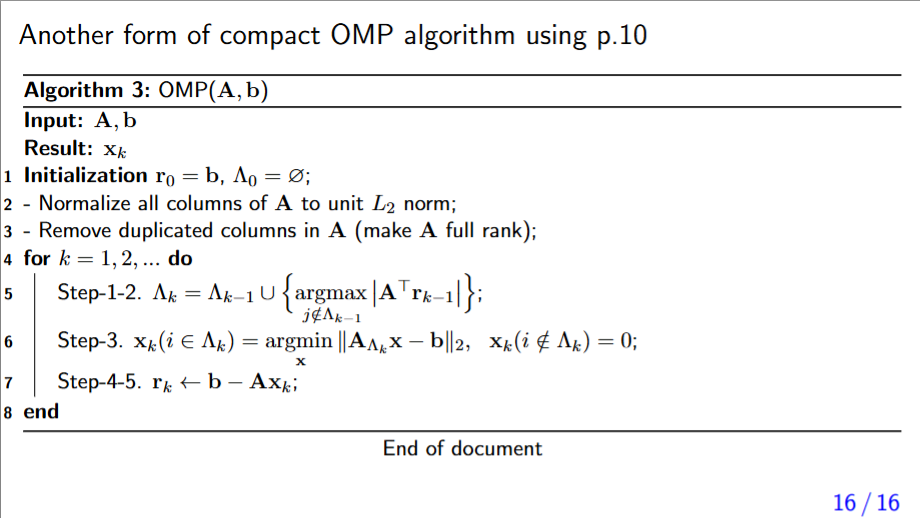
\includegraphics[width=0.8\linewidth,height=\textheight,keepaspectratio]{C:/Users/NinjaBoyASUS/OneDrive/Dokumen/Abhi/Internship/OMP-Python/omp_algorithm.png}

}

\caption{OMP Algorithm\autocite{omp-intro}}

\end{figure}%

This algorithm can be implemented in MATLAB and Python with necessary
toolboxes and libraries.

\subsection{3.1.1 Algorithm
Implementation}\label{algorithm-implementation}

\begin{itemize}
\tightlist
\item
  \textbf{MATLAB}
\end{itemize}

Here, The code is divided into two main parts: the OMP function
definition and the signal generation/reconstruction workflow. The omp
function implements the OMP algorithm. It takes as input a measurement
matrix A, a measurement vector b, and the sparsity level K. The function
normalizes the columns of A and initializes the residual r as the
measurement vector. It iteratively selects the column of A most
correlated with the current residual, adds its index to the support set
Lambda, and solves a least-squares problem to update the estimated
sparse vector x. The residual is updated accordingly. This process
repeats for K iterations, corresponding to the assumed sparsity of the
original signal. For ideal omp implementation, n,m,k are defined and a
random gaussian sensing matrix is created. then a sparse signal is
created in frequency domain and is multiplied with the sensing matrix to
create the measurements(output). Now, the omp algorithm is used to
recover the frequency domain signal back and the rreconstructed and
original signals are plotted together to check for errors. For noisy
implementation, an additional gaussian noise is generated and added to
the output measurement vector and this noisy output is given to the omp
algorithm. Then a sum of random time domain sinusoidal input was given
with \(\Psi\) as a random gaussian matrix and \(\phi\) as a inbuilt
function for dft, dftmtx(). dft was taken instead of idft since the omp
was calculated in the frequency domain. the ouput was then converted to
time domain using ifft() and was plotted.

\begin{itemize}
\item
  \textbf{Python}

  Libraries like \textbf{numpy} and \textbf{matplotlib} are imported for
  mathematical operations and plotting results respectively.

  \begin{itemize}
  \item
    \textbf{Stage 1:} The basic implementation was done by taking length
    of signal (n), number of measurements (m) and non-zero values or
    sparsity (k) as input. The sensing matrix was assumed to be filled
    with random gaussian values.
  \item
    \textbf{Stage 2:} The next stage involved taking a sum of three
    sinusoidal signals as input signal (k = 3) and it is converted to a
    more sparser domain with \textbf{Discrete Cosine Transform (DCT)}.
    The function is used by importing the \textbf{scipy} library. While
    initially k was fixed, it is then taken as an input from user. DCT
    was initially tested for a single sine wave as well as for sum of
    sine waves of different frequencies, as shown in the figure below.
  \item
    \textbf{Stage 3:} In the above stages, reconstruction was observed
    for pure signals. So, a noise (in dB) was introduced before the
    reconstruction process.
  \end{itemize}
\end{itemize}

All these stages were plotted and the error was calculated and observed.

\subsection{3.1.2 Monte-Carlo Trials}\label{monte-carlo-trials}

Monte Carlo trials are a broad class of computational algorithms that
rely on repeated random sampling to obtain numerical results. The is
used to understand the behaviour of the algorithm under change in
parameters, including sparsity, noise and number of measurements taken.
It is useful for analysis, understanding its performance for various
values of multiple inputs. In other words, this acts like a testbench
for the algorithm.

The input values were stored in a list and these were fed to the trial
algorithm. The error was calculated for a number of trials for the same
input values, and only the average error is plotted to prevent unwanted
variations in reconstruction.

\subsection{3.1.3 Observations \& Results}\label{observations-results}

\begin{itemize}
\tightlist
\item
  \textbf{MATLAB}
\end{itemize}

The algorithm was initially tested directly in frequncy domain. In its
ideal form(ie. without noise), for a low enough sparsity, the algorithm
perfectly reconstructed the frequency and the amplitude values of
compressed signal. Then, two values of noise was given(SNR=0dB and
SNR=20dB). The Algorithm was able to reconstruct the signal
near-perfectly for an SNR of 20 dB. For an SNR of 0 dB(signal
power=noise power), the results were more inaccurate, both in terms of
position on the graph(frequency) and the amplitude values.The algorithm
was able to reconstruct some parts of the signal with a fair amount of
accuracy.

\begin{figure}[H]

{\centering 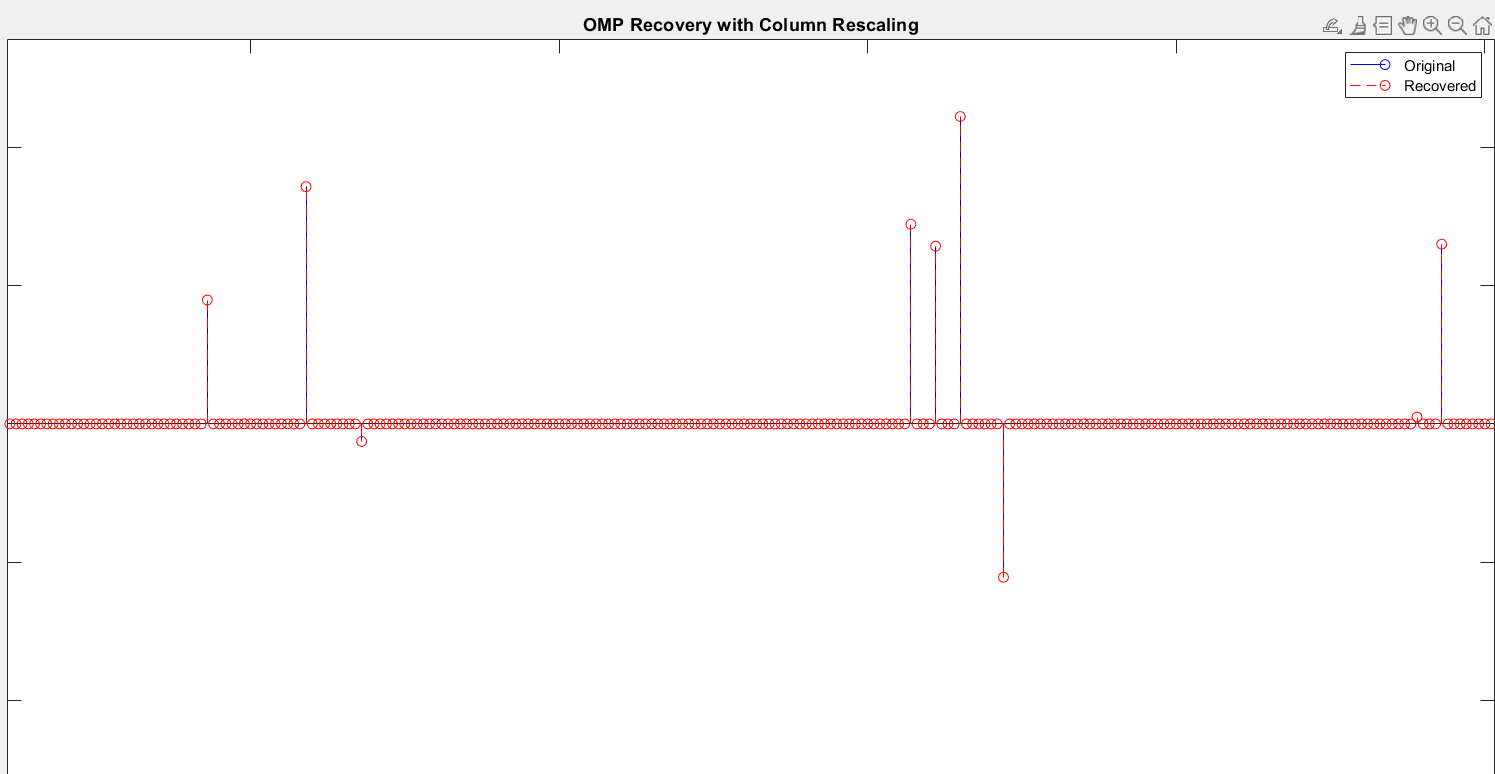
\includegraphics[width=0.8\linewidth,height=\textheight,keepaspectratio]{abar-cs_files/mediabag/omp_ideal_1.png}

}

\caption{OMP Signal Reconstruction:Ideal (No noise added)}

\end{figure}%

\begin{figure}[H]

{\centering 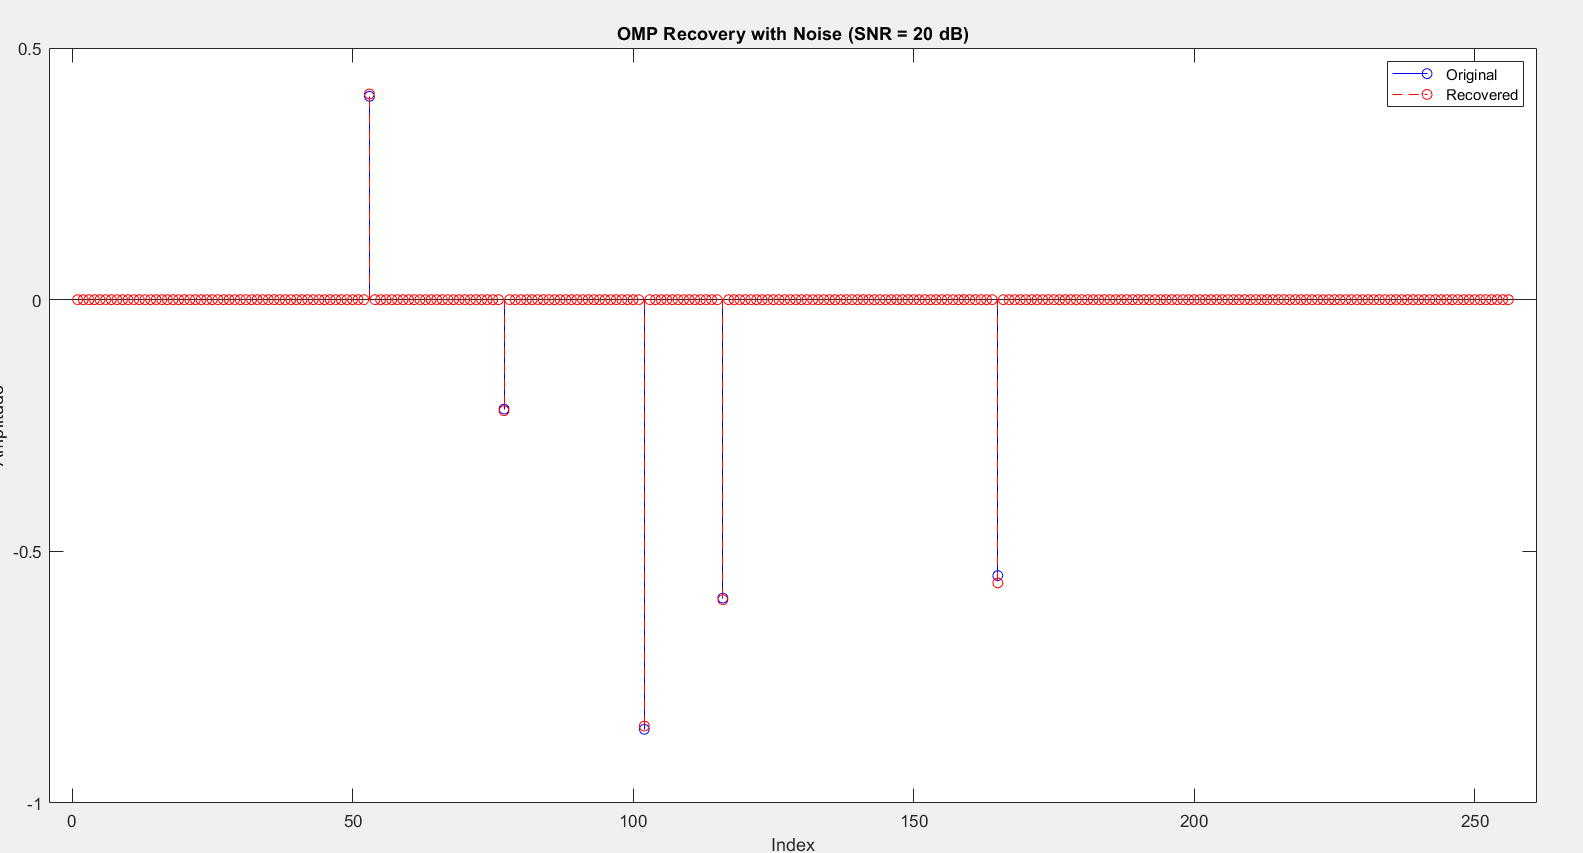
\includegraphics[width=0.8\linewidth,height=\textheight,keepaspectratio]{abar-cs_files/mediabag/omp_noisy1.png}

}

\caption{OMP Signal Reconstruction: 20dB}

\end{figure}%

\begin{figure}[H]

{\centering 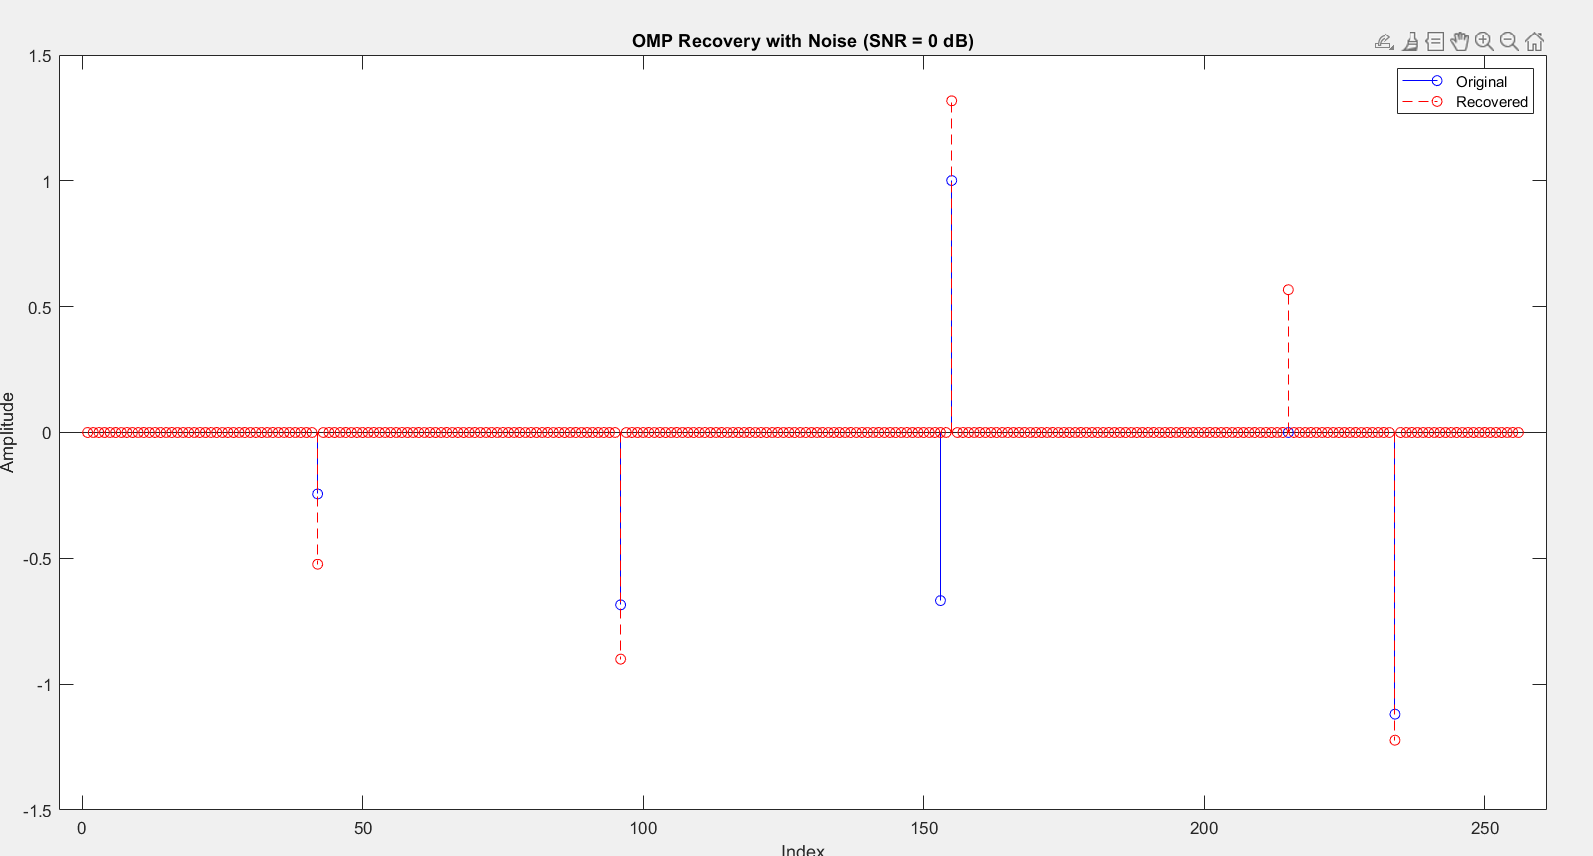
\includegraphics[width=0.8\linewidth,height=\textheight,keepaspectratio]{abar-cs_files/mediabag/omp_0db1.png}

}

\caption{OMP Signal Reconstruction: 0dB}

\end{figure}%

Next, the code was used to implement sinusoids in time domain. A sum of
5 real sinusoids was given as input to the algorithm. Then the output is
plotted along with the original signal to compare them. Initially, the
algorithm gave an output which had its amplitude greatly decreased w.r.t
the original signal.

\begin{figure}[H]

{\centering 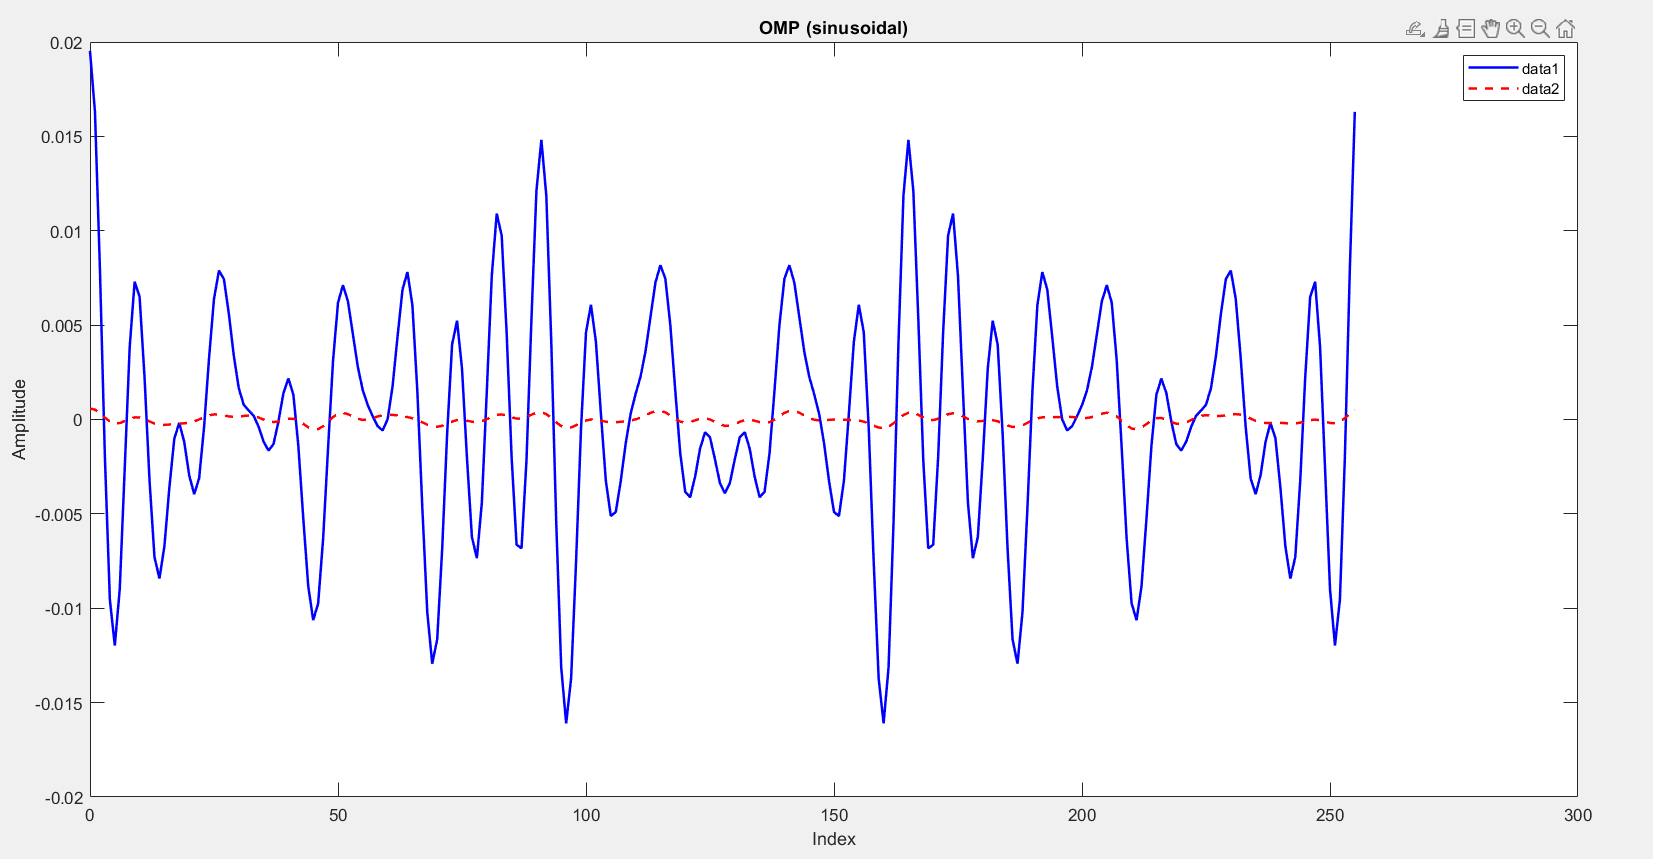
\includegraphics[width=0.8\linewidth,height=\textheight,keepaspectratio]{abar-cs_files/mediabag/omp_err_1.png}

}

\caption{OMP Signal Reconstruction: 0dB}

\end{figure}%

Further testing of the code showed the importance of normalising the
theta matrix. The normalised theta matrix showed the correct output.
After this was resolved, the algorithm was able to reconstruct the
signal fairly accurately. Smaller peaks of the input signal was harder
to reconstruct for the algorithm, and also, there was a reduction in the
amplitude of the reconstructed signal w.r.t the original signal.A slight
phase shift was observed in some outputs when the code is run for
different random inputs.

\begin{figure}[H]

{\centering 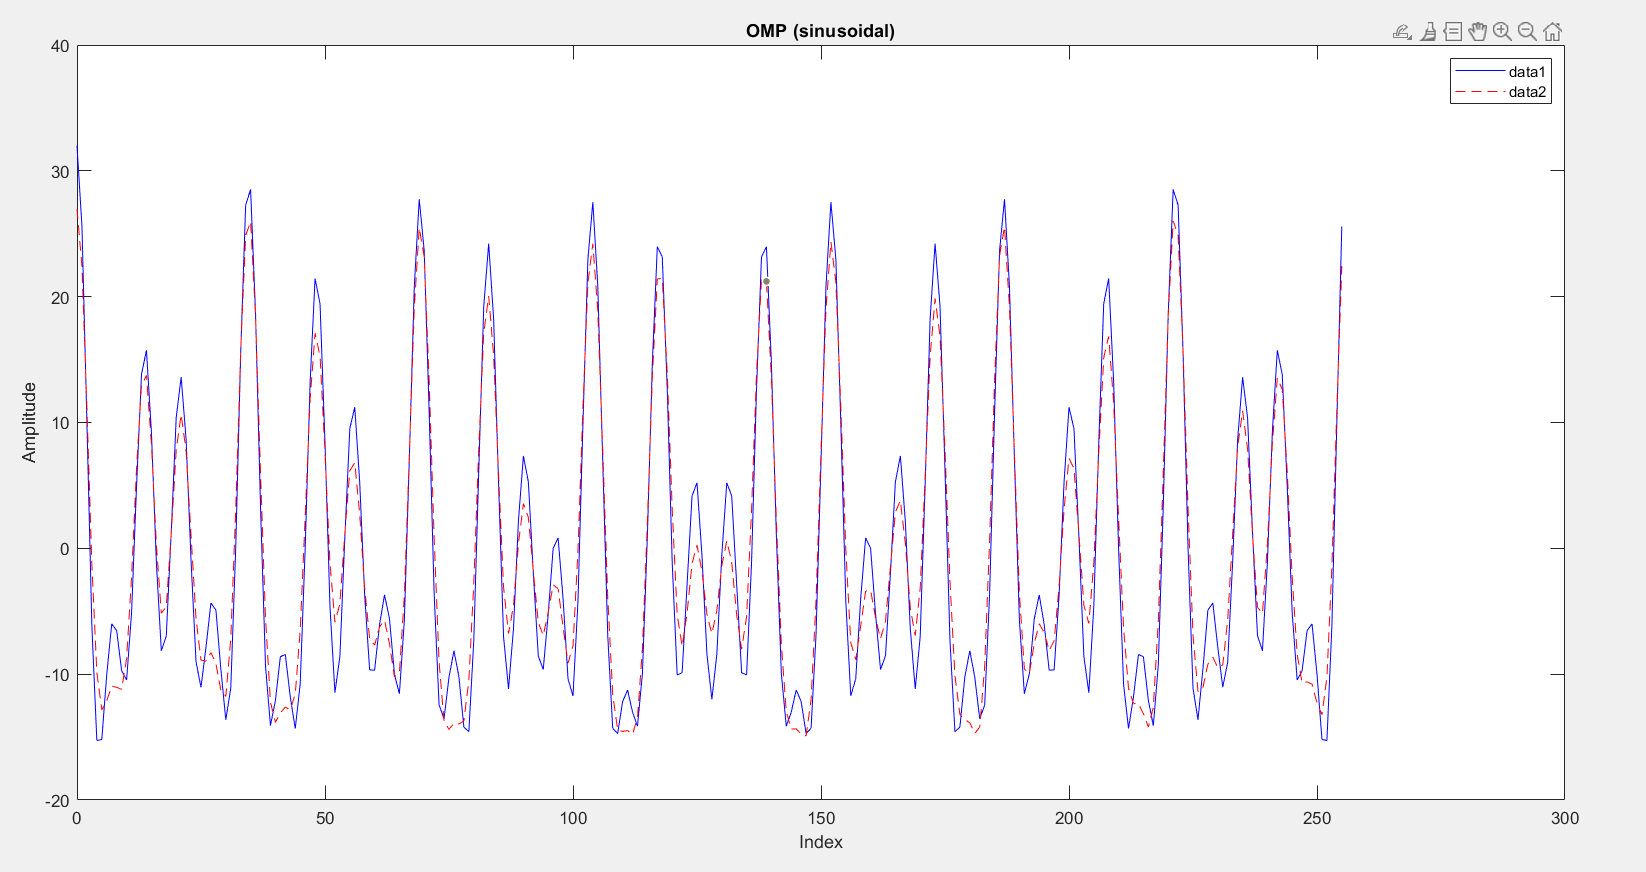
\includegraphics[width=0.8\linewidth,height=\textheight,keepaspectratio]{abar-cs_files/mediabag/omp_sine1.png}

}

\caption{OMP Signal Reconstruction: sinusoidal input}

\end{figure}%

\begin{itemize}
\tightlist
\item
  \textbf{Python}
\end{itemize}

For \textbf{Stage 1} implementation, the sparse matrix is already
created by specifying k. So, the compressed matrix (y) is generated by
just multiplying sensing matrix (\(\Theta\)) and the generated sparse
matrix (s). The results are plotted as shown below,

\begin{figure}[H]

{\centering 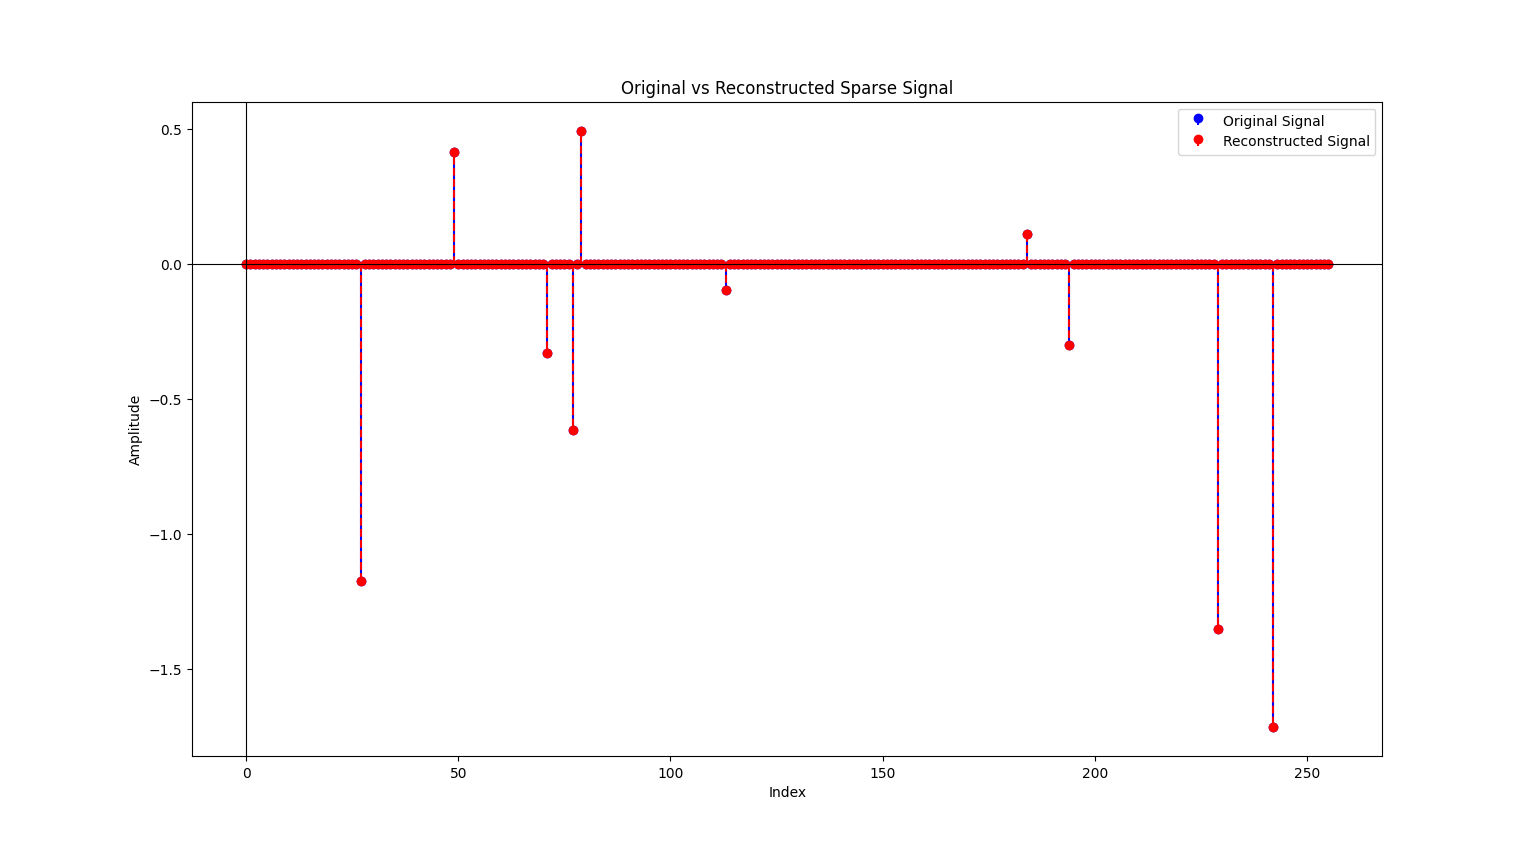
\includegraphics[width=0.8\linewidth,height=\textheight,keepaspectratio]{abar-cs_files/mediabag/omp-alg-256.png}

}

\caption{OMP Algorithm Stage 1 Implementation: Perfect Reconstruction}

\end{figure}%

While the reconstruction as shown above is very accurate, it is not
always the case. As sparsity increases, the measurements to be taken
also increases. Hence, there are some necessary conditions for perfect
recovery of a signal. As mentioned in \autocite{rani-cs}, the relation
between n, m and k is:-

\begin{equation}
\boxed{
    m \geq C \cdot k \cdot \log\left(\frac{n}{k}\right)
}
\end{equation}

where \textbf{C} is a constant almost equal to 2.

Hence, if the above equation is not satisfied, then reconstruction is
very difficult. The failed reconstruction is shown below.

\begin{figure}[H]

{\centering 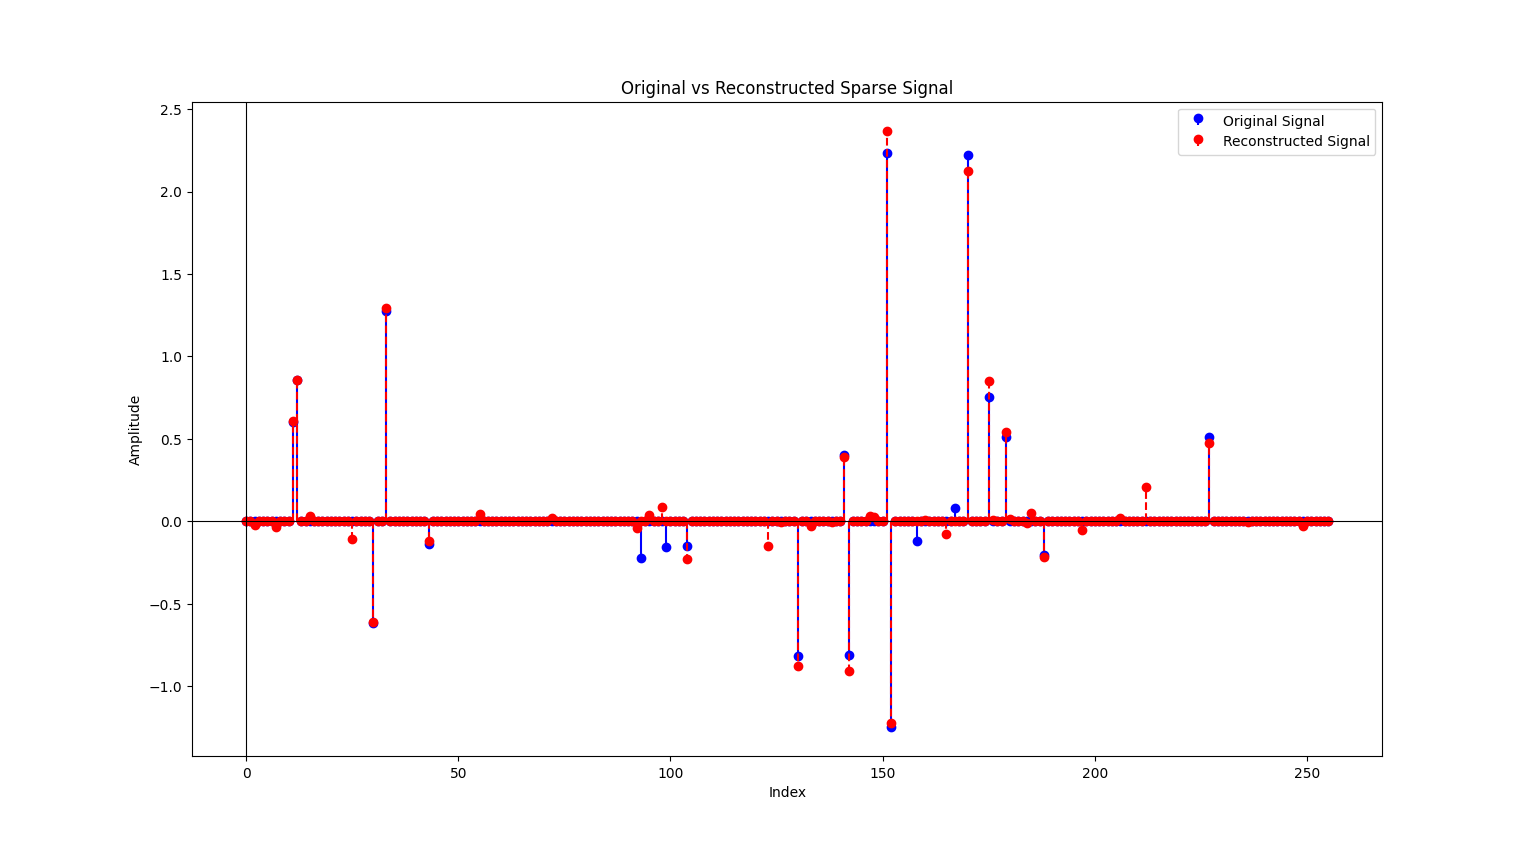
\includegraphics[width=0.8\linewidth,height=\textheight,keepaspectratio]{abar-cs_files/mediabag/omp-alg-2561.png}

}

\caption{OMP Algorithm Stage 1 Implementation: Failed Reconstruction}

\end{figure}%

When it comes to \textbf{Stage 2} implementation, the sensing matrix is
divided into a basis matrix and measurement matrix. The basis matrix is
used to convert our input signal to a sparser signal. For sinusoidal
inputs, it is best to represent the signals in its frequency domain. So,
FFT or DCT can be used. Since, all sinusoids are real signals, DCT was
possible. The sum of sinusoids were converted to DCT and the results are
being plotted to check its sparsity.

\begin{figure}[H]

{\centering 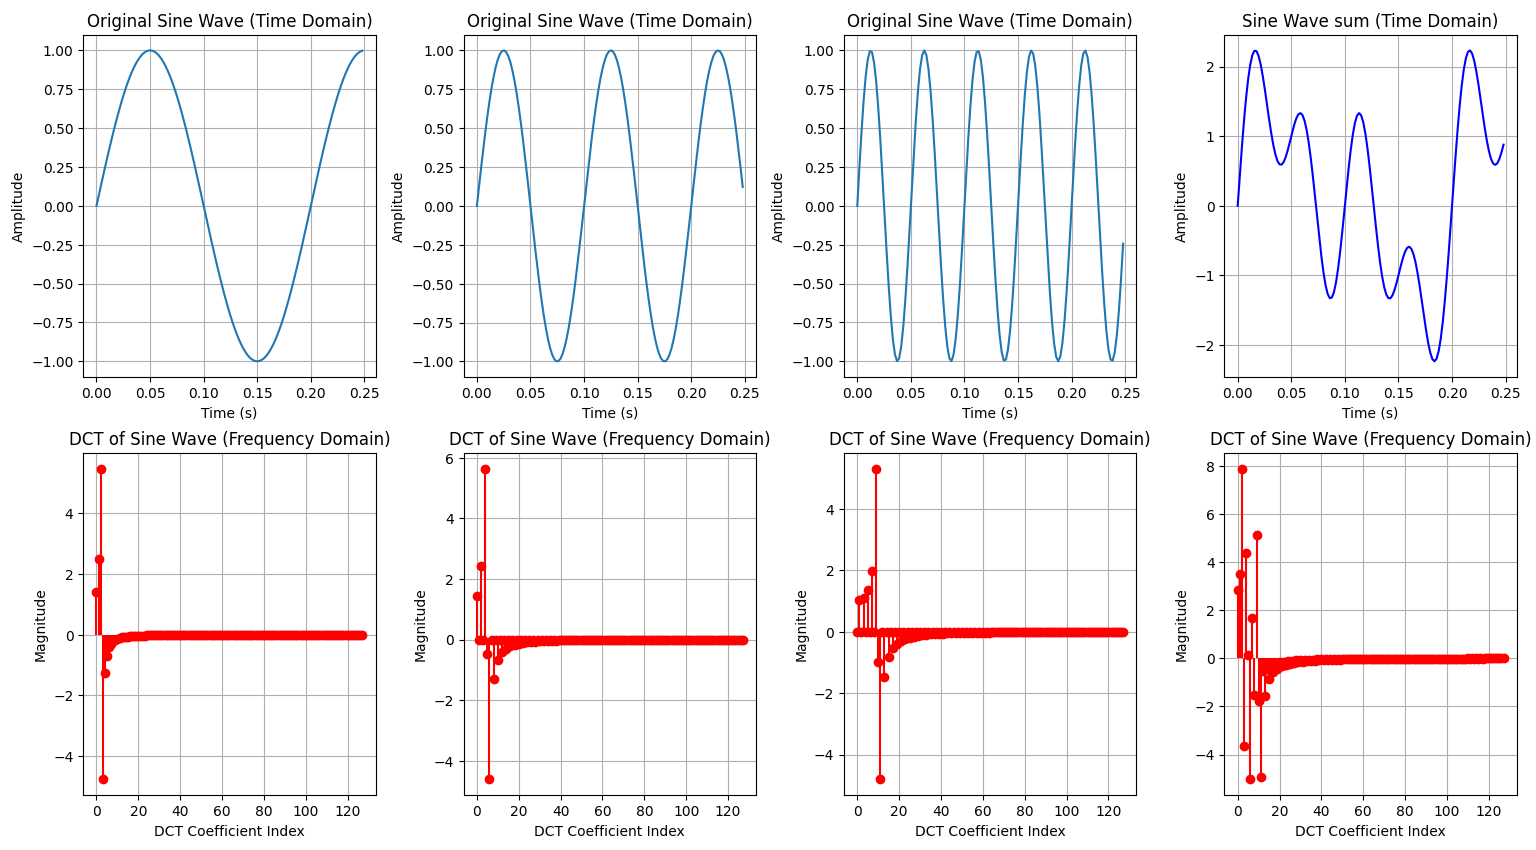
\includegraphics[width=0.8\linewidth,height=\textheight,keepaspectratio]{abar-cs_files/mediabag/sine-dct.png}

}

\caption{OMP Algorithm Stage 2 Implementation: DCT Basis on Sinusoidal
signals}

\end{figure}%

The sinusoidal signal is initially tested for various values of n and m,
keeping k = 3. Some of the results are plotted as shown,

\begin{figure}[H]

{\centering 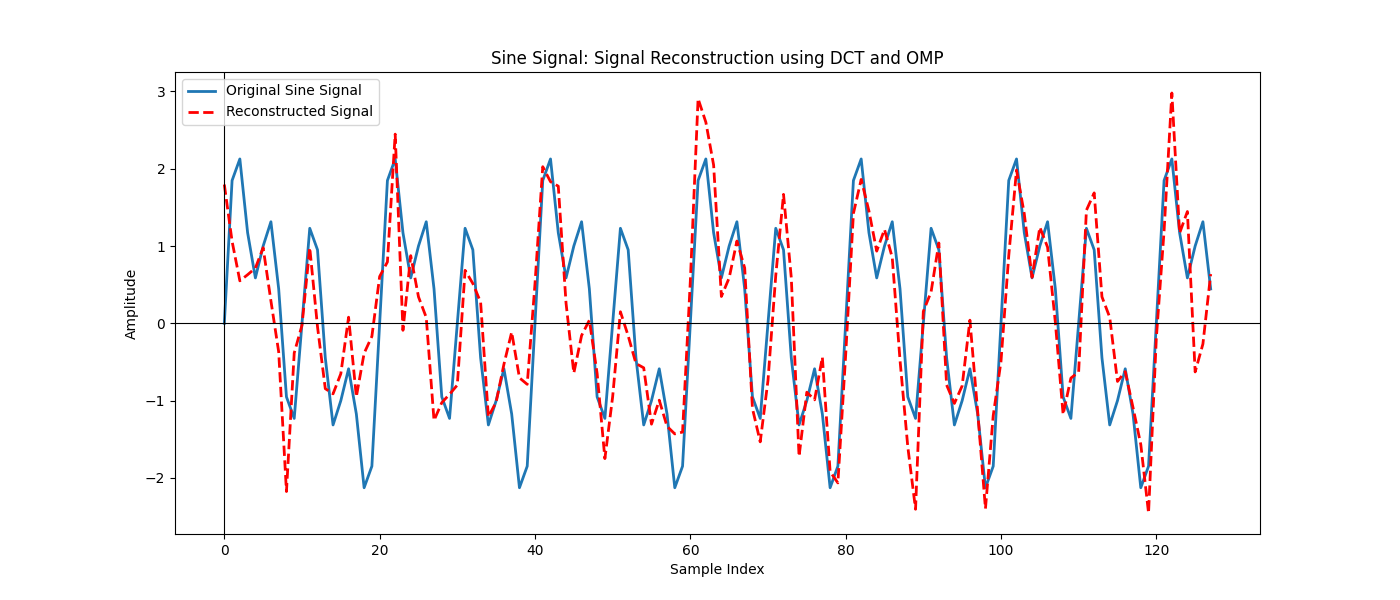
\includegraphics[width=0.8\linewidth,height=\textheight,keepaspectratio]{abar-cs_files/mediabag/omp-sine-n128-m60.png}

}

\caption{OMP Algorithm Stage 2 Implementation: For n = 128, m = 60}

\end{figure}%

\begin{figure}[H]

{\centering 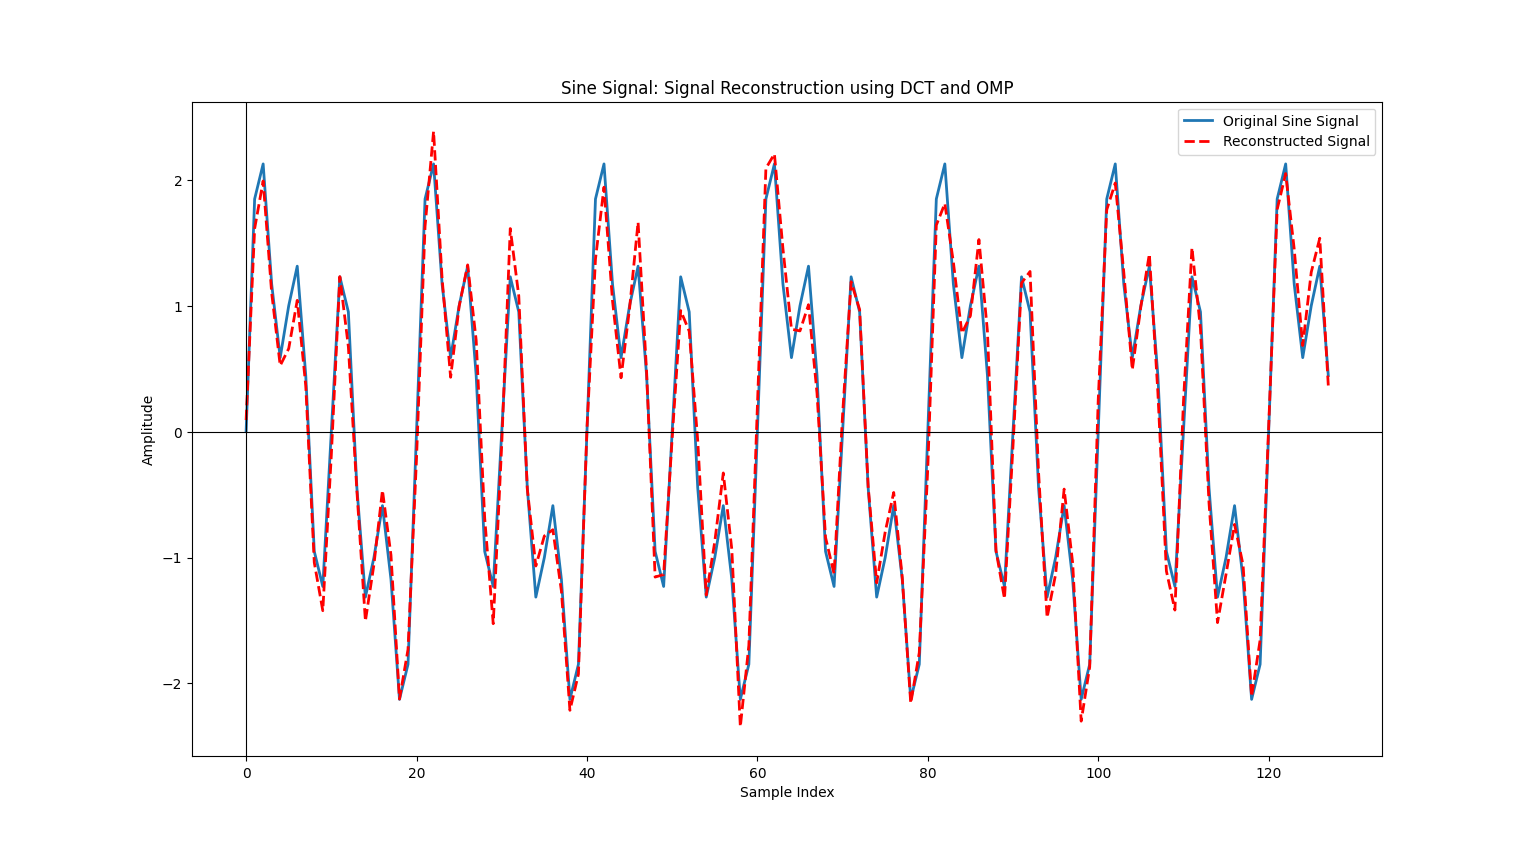
\includegraphics[width=0.8\linewidth,height=\textheight,keepaspectratio]{abar-cs_files/mediabag/omp-sine-n128-m100.png}

}

\caption{OMP Algorithm Stage 2 Implementation: For n = 128, m = 100}

\end{figure}%

So, generally we can say as \textbf{number of measurements increases,
the reconstruction error decreases}. Till now, no noise has been
considered during the reconstruction. To analyse the algorithm for each
value of n, m, k and even noise, it is difficult for us to understand
the trend of error. So, a Monte Carlo trial has been implemented on the
OMP algorithm for three variable parameters, \textbf{measurements},
\textbf{sparsity} and \textbf{noise}. So, all three parameters are
compared and the results are plotted.

\begin{figure}[H]

{\centering 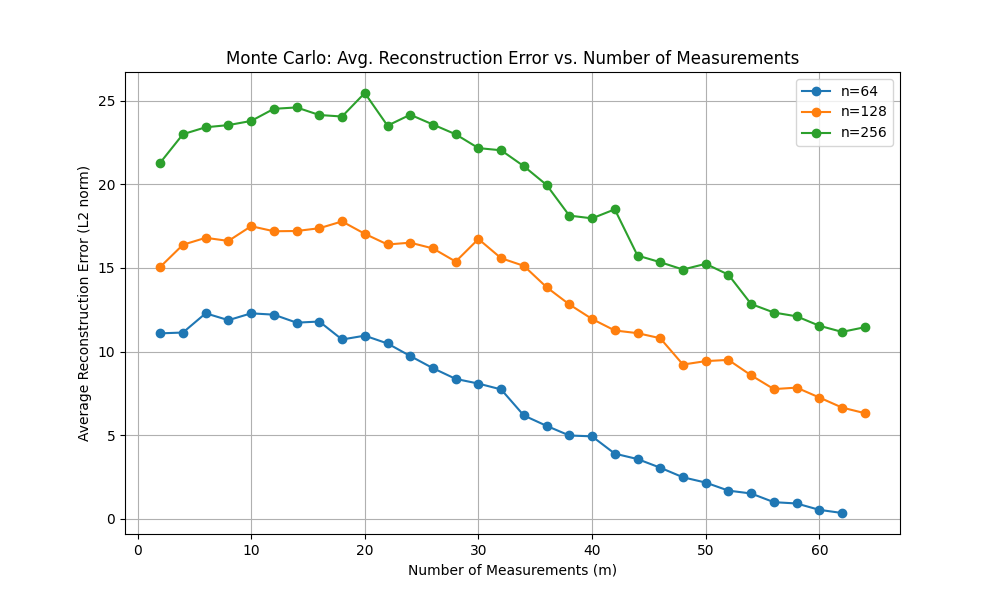
\includegraphics[width=0.8\linewidth,height=\textheight,keepaspectratio]{abar-cs_files/mediabag/omp-montecarlo-sum.png}

}

\caption{Monte Carlo Trial: Measurements (m)}

\end{figure}%

The analysis above is for noiseless, fixed sparsity (k = 3)
reconstruction.

\begin{figure}[H]

{\centering 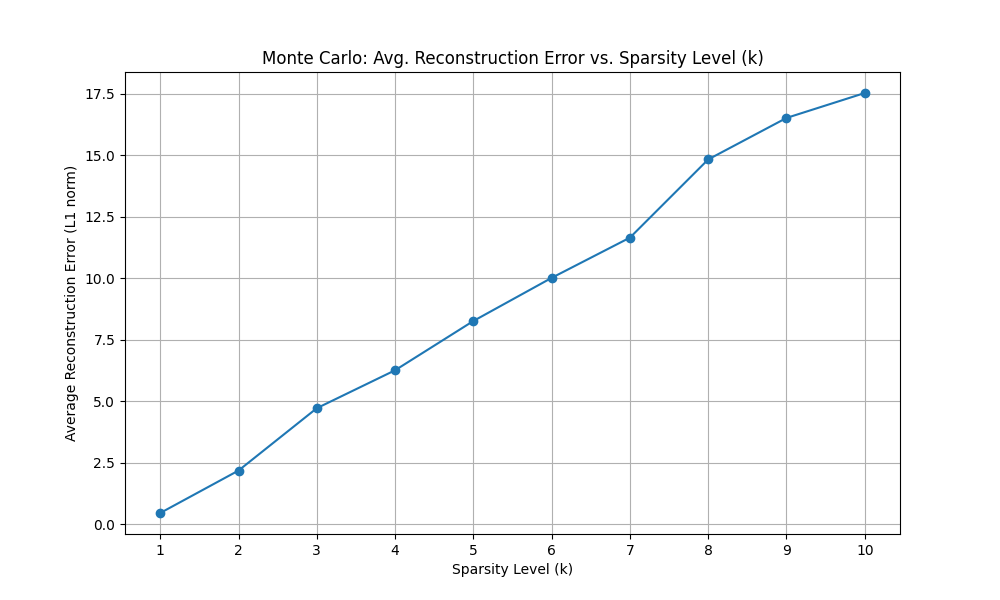
\includegraphics[width=0.8\linewidth,height=\textheight,keepaspectratio]{abar-cs_files/mediabag/omp-montecarlo-spars.png}

}

\caption{Monte Carlo Trial: Sparsity (k)}

\end{figure}%

\begin{figure}[H]

{\centering 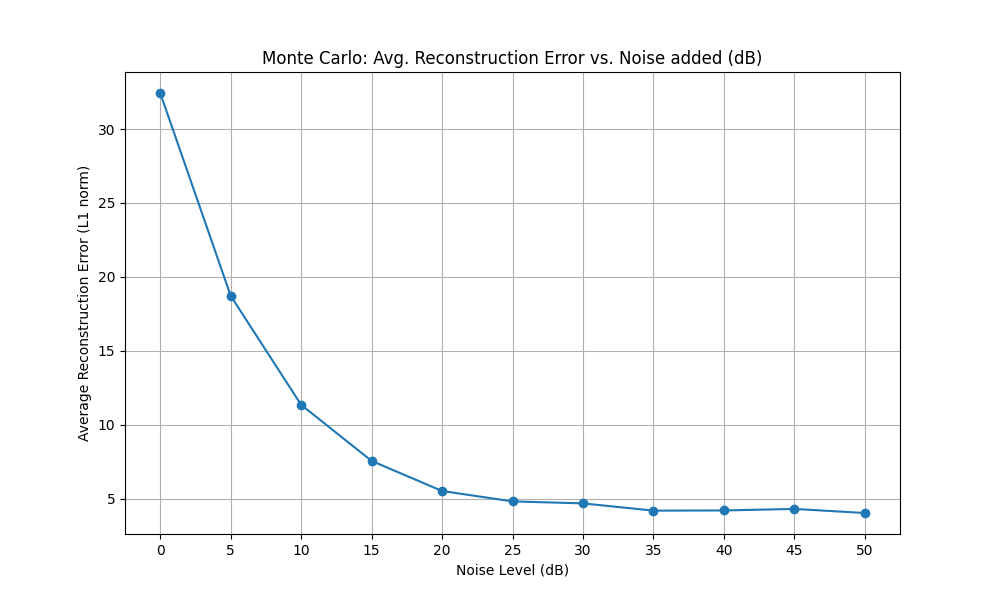
\includegraphics[width=0.8\linewidth,height=\textheight,keepaspectratio]{abar-cs_files/mediabag/omp-montecarlo-noise.png}

}

\caption{Monte Carlo Trial: Noise (in dB)}

\end{figure}%

In summary, OMP is a robust and efficient algorithm for compressed
sensing when the signal is sparse and the measurement conditions are
favorable. However, its sensitivity to noise and the need for sufficient
measurements must be considered in practical applications.

\subsection{3.2 ITERATIVE SHRINKAGE THRESHOLDING ALGORITHM
(ISTA)}\label{iterative-shrinkage-thresholding-algorithm-ista}

The ISTA is an iterative, convex optimisation method for solving sparse
signal recovery problems, particularly those formulated as LASSO or
basis pursuit denoising. ISTA iteratively updates the solution by
applying a gradient descent step followed by a soft-thresholding
(shrinkage) operation to promote sparsity. The general steps are:

\begin{enumerate}
\def\labelenumi{\arabic{enumi}.}
\tightlist
\item
  Initialize the sparse coefficient vector.
\item
  At each iteration, perform a gradient descent step to minimize the
  data fidelity term.
\item
  Apply the soft-thresholding operator to enforce sparsity.
\item
  Repeat until convergence.
\end{enumerate}

These steps are as shown, from

\begin{figure}[H]

{\centering \includegraphics[width=0.8\linewidth,height=\textheight,keepaspectratio]{abar-cs_files/mediabag/.pdf}

}

\caption{ISTA Algorithm\autocite{fast-sparse-coding}}

\end{figure}%

\subsubsection{3.2.1 Algorithm Implementation \& Monte Carlo
Trial}\label{algorithm-implementation-monte-carlo-trial}

Just like in OMP implemntation, the basic libraries were imported and
the sinusoidal input is converted to its sparser domain using DCT. The
soft thresholding function plays a role in enforcing sparsity by
shrinking very small values to zero. Since convergence is very slow in
ISTA, the number of iterations are higher than that of OMP.

Monte Carlo has been implemented in a very similar manner as that of OMP
and it has been checked for all the 3 paramters. Moreover, both the
algorithms have been compared for these parameters, and their
performance has been observed and analysed.

\subsubsection{3.2.2 Observations \&
Results}\label{observations-results-1}

Implementing ISTA for a sinusoidal input had some similarities with that
of the OMP algorithm. The trends in the major 3 parameters are same for
both the algorithms. Initially ISTA was checked for pure reconstruction,
that is no noise interfernce. The result is as plotted,

\begin{figure}[H]

{\centering \includegraphics[width=0.8\linewidth,height=\textheight,keepaspectratio]{abar-cs_files/mediabag/.pdf}

}

\caption{ISTA Algorithm Implementation (Ideal)}

\end{figure}%

It is observed that as the number of iterations for ISTA increases, the
error decreases.

Now, when noise is added during the process, its performance is also as
shown,

\begin{figure}[H]

{\centering \includegraphics[width=0.8\linewidth,height=\textheight,keepaspectratio]{abar-cs_files/mediabag/.pdf}

}

\caption{ISTA Algorithm Implementation (With Noise)}

\end{figure}%

Here, unlike OMP, ISTA is very resistant to noise variation and hence
explains its advantage over OMP. That is because of the shrinkage
function, which shrinks small coefficients to zero and its
regularisation term penalises the high variance solutions. In contrary,
OMP being a greedy algorithm, tends to select the noisy atoms causing to
succumb to the effect of noise. Hence, ISTA is more robust to noise than
OMP.

The Monte Carlo for ISTA has been implemented with varying measurements
for every value of n.~The results are to some extent similar to that of
the OMP, that is the reconstruction error follows an inverse
relationship with the number of measurements, which is as shown below,

\begin{figure}[H]

{\centering 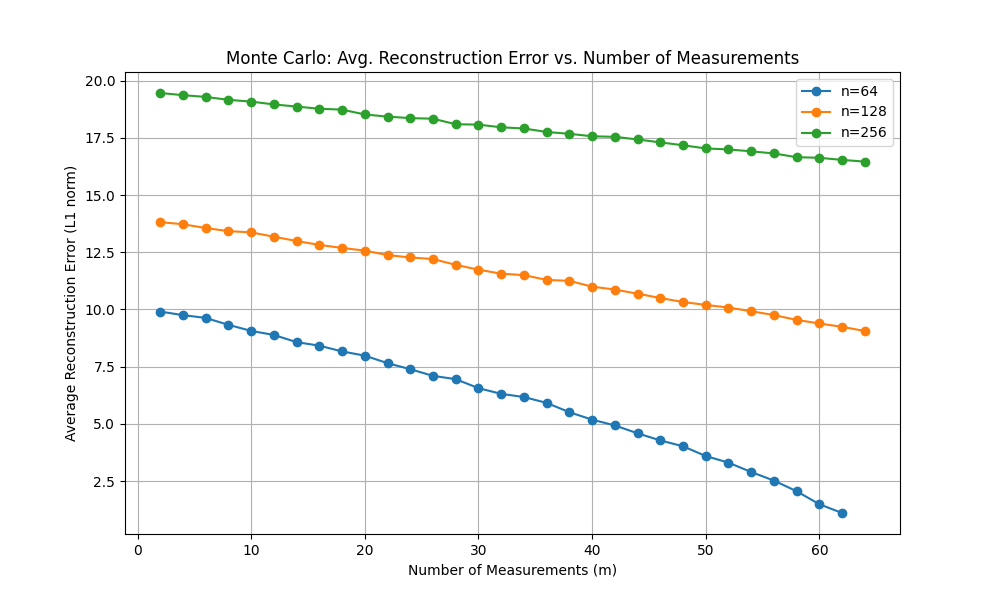
\includegraphics[width=0.8\linewidth,height=\textheight,keepaspectratio]{abar-cs_files/mediabag/istaa-montecarlo.png}

}

\caption{Monte Carlo Trial: Measurements (m)}

\end{figure}%

With these 3 parameters used for the trial, it can be done to compare
both ISTA and OMP. This is done so as to assess and understand the scope
of the algorithm for future work, etc. The comparisons are shown below

\begin{figure}[H]

{\centering 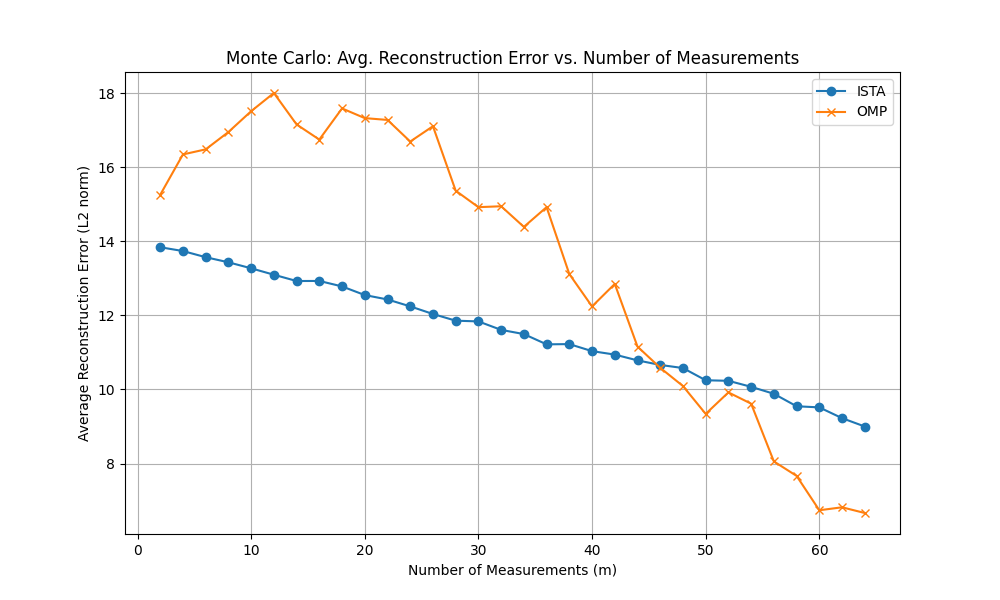
\includegraphics[width=0.8\linewidth,height=\textheight,keepaspectratio]{abar-cs_files/mediabag/montecarlo-omp-ista-.png}

}

\caption{OMP v/s ISTA (m)}

\end{figure}%

\begin{figure}[H]

{\centering \includegraphics[width=0.8\linewidth,height=\textheight,keepaspectratio]{abar-cs_files/mediabag/montecarlo-omp-ista-1.png}

}

\caption{OMP v/s ISTA (noise)}

\end{figure}%

\begin{figure}[H]

{\centering 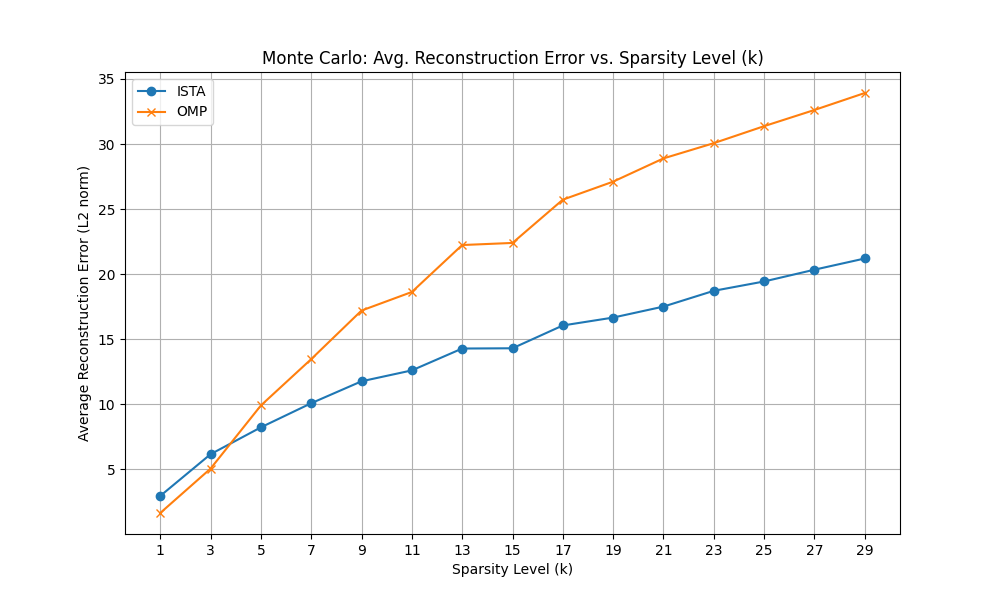
\includegraphics[width=0.8\linewidth,height=\textheight,keepaspectratio]{abar-cs_files/mediabag/montecarlo-omp-ista-12.png}

}

\caption{OMP v/s ISTA (sparsity)}

\end{figure}%

In summary, both OMP and ISTA have their own strengths and are suitable
for different scenarios in compressed sensing-based radar signal
processing:

\begin{itemize}
\item
  \textbf{OMP} excels when the signal is highly sparse and the number of
  measurements is sufficient. It is computationally efficient and
  provides accurate reconstruction in low-noise environments. However,
  its performance degrades with increased noise or when the sparsity
  assumption is violated.
\item
  \textbf{ISTA} is more robust to noise due to its regularization and
  shrinkage steps. It can handle less sparse signals and noisy
  measurements better than OMP, albeit at the cost of slower convergence
  and higher computational complexity. It is best in handling
  undersampled and noisy data.
\end{itemize}

The choice between OMP and ISTA depends on the specific requirements of
the application, such as the expected sparsity of the signal, noise
levels, and computational resources. In practice, a trade-off must be
made between reconstruction accuracy, noise robustness, and
computational efficiency.

\subsection{3.3 COORDINATE DESCENT (CoD)}\label{coordinate-descent-cod}

Coordinate Descent is a simple yet powerful optimization algorithm that
is widely used in compressed sensing applications, especially for
solving large-scale sparse recovery problems such as LASSO (Least
Absolute Shrinkage and Selection Operator). It works by minimizing (or
maximizing) a function by solving for one variable at a time while
keeping the others fixed. The process repeats, cycling through each
variable (or ``coordinate'') in turn, updating its value to reduce the
objective function. The general steps are: 1. Initialize the sparse
coefficient vector. 2. For each coordinate (variable), update its value
by minimizing the objective function with respect to that coordinate,
keeping all other variables fixed. 3. Apply the soft-thresholding
operator to the updated coordinate to enforce sparsity. 4. Repeat steps
2 and 3 for all coordinates, cycling through them until convergence.

\begin{center}
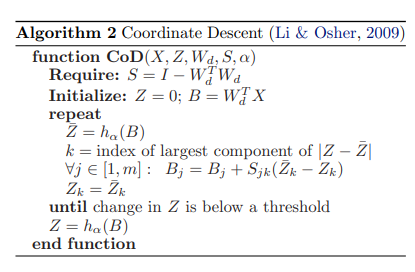
\includegraphics[width=0.8\linewidth,height=\textheight,keepaspectratio]{abar-cs_files/mediabag/algorithm_cod.png}
\end{center}

\subsubsection{3.3.1 Algorithm
Implementation}\label{algorithm-implementation-1}

In the MATLAB implementation of CoD algorithm, The process begins by
generating a sparse signal (z\_true) and its measurement (y) using a
random sensing matrix (Phi). The main loop iteratively updates each
coordinate of the sparse coefficient vector (z) by applying the
soft-thresholding operator, which enforces sparsity. At each iteration,
the coordinate with the largest change is selected and updated to
minimize the objective function. The reconstructed signal is then
compared to the original, and the mean squared error (MSE) is tracked
over iterations to monitor convergence. The code concludes by plotting
both the original and reconstructed signals, as well as the MSE
progression, illustrating the effectiveness of the CoD algorithm in
recovering sparse signals.

\subsubsection{3.3.2 Monte Carlo Trials}\label{monte-carlo-trials-1}

A python script was created for the algorithm that closely matches the
MATLAB implementation and Monte Carlo Trials were conducted on the
algorithm. The input values were stored in a list and these were fed to
the trial algorithm. The error was calculated for a number of trials for
the same input values, and only the average error is plotted to prevent
unwanted variations in reconstruction.

\subsubsection{3.3.3 Observations \&
Results}\label{observations-results-2}

Two types of implementations were considered- an ideal noiseless input
signal and an input signal with 10dB of noise. For the ideal condition,
multple values of m were considered(32,64 and 128) for n = 128 and the
original vs reconstructed signal graphs were plotted.

\begin{figure}[H]

{\centering \includegraphics[width=0.8\linewidth,height=\textheight,keepaspectratio]{abar-cs_files/mediabag/cod_m32.png}

}

\caption{Ideal CoD at m = 32}

\end{figure}%

\begin{figure}[H]

{\centering \includegraphics[width=0.8\linewidth,height=\textheight,keepaspectratio]{abar-cs_files/mediabag/cod_m64.png}

}

\caption{Ideal CoD at m = 64}

\end{figure}%

\begin{figure}[H]

{\centering \includegraphics[width=0.8\linewidth,height=\textheight,keepaspectratio]{abar-cs_files/mediabag/cod_m128.png}

}

\caption{Ideal CoD at m = 128}

\end{figure}%

Also, the plot between the Mean Squared Error(MSE) and the number of
iterations gives us the convergence of the algorithm.

\begin{figure}[H]

{\centering 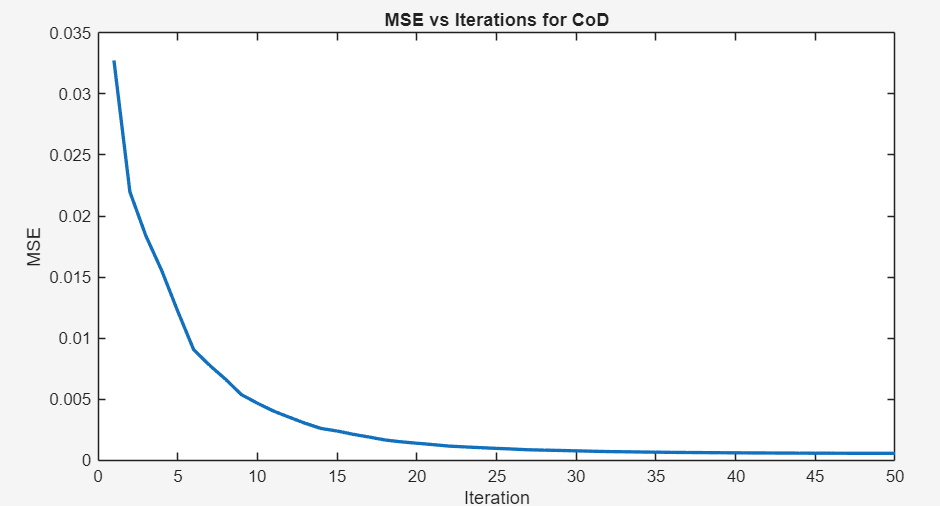
\includegraphics[width=0.8\linewidth,height=\textheight,keepaspectratio]{abar-cs_files/mediabag/cod_conv_ideal.png}

}

\caption{Iterations vs MSE plot for Ideal CoD}

\end{figure}%

it is observed that increase in resolution, ie. increasing the value of
m increases the accuracy of the reconstructed signal. The accuracy is
more than enough for m = 32, which is only one fourth of the total
samples. at m = 64, the signals is almost entirely reconstructed except
for a slight decrease in Amplitude.

Now, for the noisy implementation m = 32 and 64 were considered for n =
128 and the corresponding graphs were plotted.

\begin{figure}[H]

{\centering 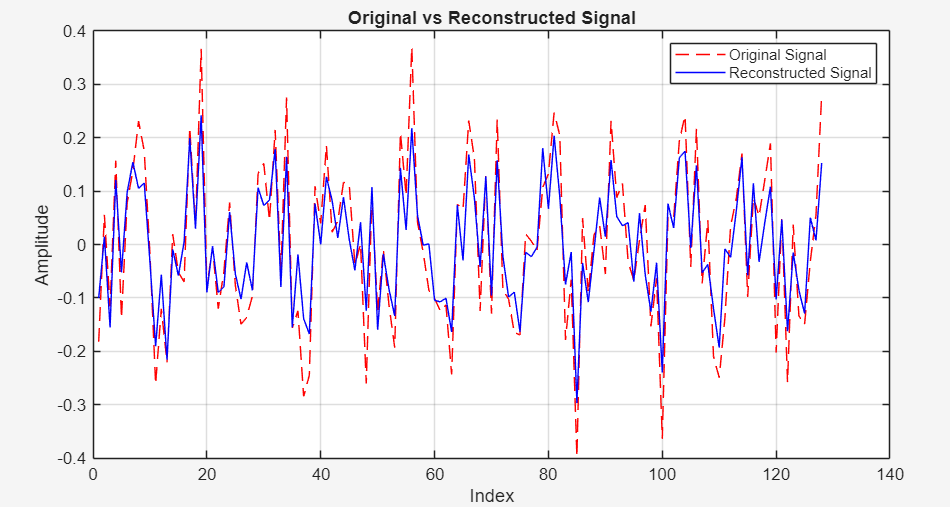
\includegraphics[width=0.8\linewidth,height=\textheight,keepaspectratio]{abar-cs_files/mediabag/cod_m32_noisy1.png}

}

\caption{Original vs Reconstructed signal: m=32}

\end{figure}%

\begin{figure}[H]

{\centering \includegraphics[width=0.8\linewidth,height=\textheight,keepaspectratio]{abar-cs_files/mediabag/cod_m32_noisy_mse.png}

}

\caption{Iterations vs MSE graph: m = 32}

\end{figure}%

\begin{figure}[H]

{\centering \includegraphics[width=0.8\linewidth,height=\textheight,keepaspectratio]{abar-cs_files/mediabag/cod_m64_noisy1.png}

}

\caption{Original vs Reconstructed signal: m=64}

\end{figure}%

\begin{figure}[H]

{\centering 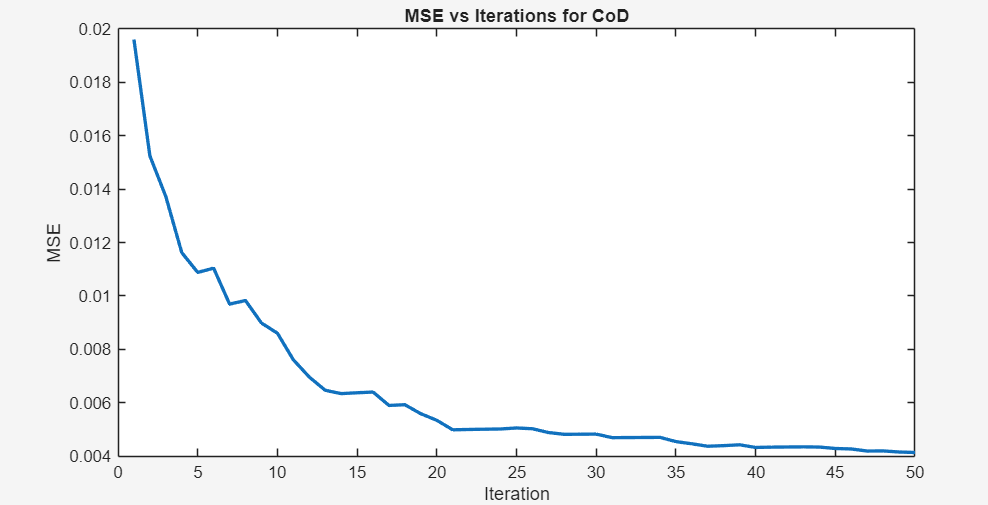
\includegraphics[width=0.8\linewidth,height=\textheight,keepaspectratio]{abar-cs_files/mediabag/cod_m64_noisy_mse.png}

}

\caption{Iterations vs MSE graph: m = 64}

\end{figure}%

for noisy implementation, n = 32 shows considerable error in amplitudes.
Some of the smaller peaks are ignored by the algorithm. Its Iteration vs
MSE graph is spiky but still shows a clear trend of convergence. n = 64
shows even better performance. There are still some amplitude errors,
but this is very good performance for only half the samples. The
Iteration vs MSE graph is much more smooth. Overall, the algorithm is
more than capable of reconstructing a noisy signal of low resolution
with managable errors. The Monte Carlo for CoD has been implemented in
the same way as for OMP and ISTA, with varying measurements for every
value of n.

\begin{figure}[H]

{\centering 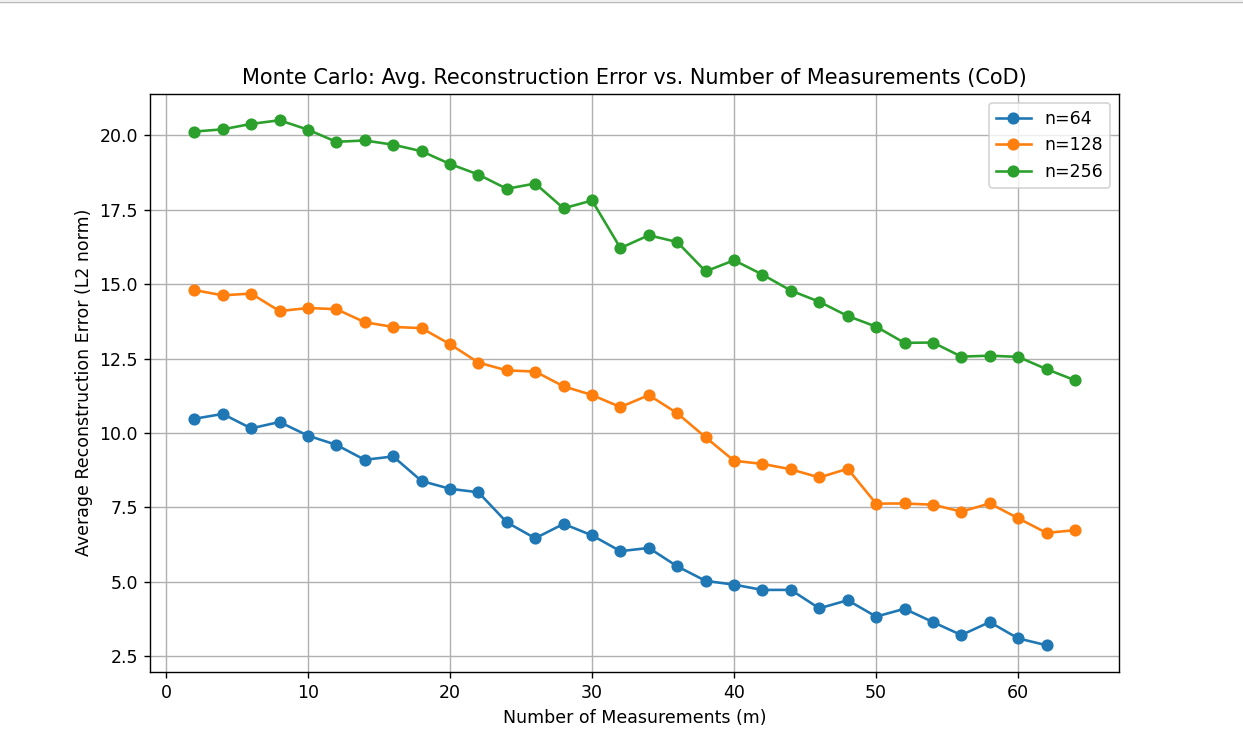
\includegraphics[width=0.8\linewidth,height=\textheight,keepaspectratio]{abar-cs_files/mediabag/montecarlo_CoD.png}

}

\caption{Monte Carlo Trials - CoD}

\end{figure}%

The results show that the reconstruction error is inversely proportional
to the number of measurements m and proportional to the length n.

\newpage

\mainsection{CHAPTER 4: REAL TIME PROCESSING OF RADAR SIGNALS}

The algorithms discussed above, such as OMP, ISTA, and CoD, generally
have computational complexities that scale quadratically or cubically
with the problem size. For example, OMP has a worst-case time complexity
of cubic terms per signal. ISTA and CoD, while sometimes more efficient
per iteration, may require a large number of iterations to converge,
leading to overall quadratic or higher complexity.

So, hence, while these algorithms are effective for offline or simulated
environments, they are often not sufficient for real-time radar signal
processing due to several reasons:

\begin{itemize}
\item
  \textbf{Computational Complexity:} Algorithms like OMP, ISTA, and CoD
  can be computationally intensive, especially for large-scale problems
  or high-dimensional signals. Real-time radar applications require fast
  processing to meet strict latency requirements, which may not be
  achievable with these iterative algorithms on standard hardware.
\item
  \textbf{Latency Constraints:} Real-time systems demand immediate or
  near-instantaneous responses. The iterative nature of these algorithms
  can introduce unacceptable delays, making them unsuitable for
  time-critical radar applications.
\item
  \textbf{Resource Limitations:} Embedded radar systems often have
  limited memory and processing power. The memory and computational
  requirements of these algorithms may exceed the capabilities of such
  systems.
\item
  \textbf{Robustness to Dynamic Environments:} Real-time radar must
  handle rapidly changing environments, interference, and noise. The
  algorithms discussed may not adapt quickly enough to such variations
  or may require parameter tuning that is impractical in real time.
\item
  \textbf{Scalability:} As the number of targets or the dimensionality
  of the data increases, the performance of these algorithms can
  degrade, further limiting their applicability in real-time scenarios.
\end{itemize}

To address these challenges, we are introducing two modifications in our
model,

\begin{enumerate}
\def\labelenumi{\arabic{enumi}.}
\item
  \textbf{Augmented Dictionary for Blind Reconstruction}
\item
  \textbf{Reconstruction Algorithm Unrolling}
\end{enumerate}

\newpage

\mainsection{CHAPTER 5: BLIND RECONSTRUCTION USING AUGMENTED DICTIONARY}

\subsection{5.1 INTRODUCTION}\label{introduction-2}

In traditional compressed sensing, the measurement process assumes prior
knowledge of the basis (or dictionary) in which the signal is sparse.
However, in many real-world radar applications, the exact basis or the
parameters of the signal (such as frequency, phase, or waveform) may not
be known in advance. This scenario is referred to as \textbf{blind
reconstruction}.

Blind reconstruction aims to recover both the sparse signal and the
underlying dictionary (or its parameters) from the compressed
measurements. One effective approach to address this challenge is to use
an \textbf{augmented dictionary}--- a collection of candidate basis
vectors that span a wider range of possible signal structures.

So, the upcoming sections will discuss the implementation and the
observations drawn from it.

\subsection{5.2 IMPLEMENTATION}\label{implementation}

In the previous implementations, the input signal type is known and
hence, the basis is also known and the compression is done with ease.
But in real life, the the radar can receive any type of signals, and
some of them might not be sparse enough for the signal to be taken for
reconstruction.

For now, only 3 types of signals are accepted as inputs, that is
\textbf{Single tone Sinusoids}, \textbf{LFM(Linear Frequency Modulated)}
a.k.a \textbf{Chirp signals} and \textbf{BPSK (Binary Phase Shifted
Key)} signals. The input signals are generated and is sent through a
mixer. The suitable basis is analysed and selected for making the
augmented basis by concatenating each of the individual dictionaries.

\begin{equation}
\boxed{
    \Psi_{\text{aug}} = \left[\, \Psi_{\text{sinusoid}} \;\Big|\; \Psi_{\text{LFM}} \;\Big|\; \Psi_{\text{BPSK}} \,\right]
}
\end{equation}

where \(\Psi_{\text{sinusoid}}\), \(\Psi_{\text{LFM}}\), and
\(\Psi_{\text{BPSK}}\) are the basis matrices for Single-tone sinusoids,
LFM signals, and BPSK signals, respectively, and \(\Psi_{\text{aug}}\)
is the augmented dictionary formed by concatenating these bases.

A gaussian noise is also added to check its performance in noisy
environments.

\subsection{5.3 OBSERVATIONS \& RESULTS}\label{observations-results-3}

Initially the DCT matrix is used as the basis for the above mentioned
input signals and their results are as shown,

\begin{figure}[H]

{\centering 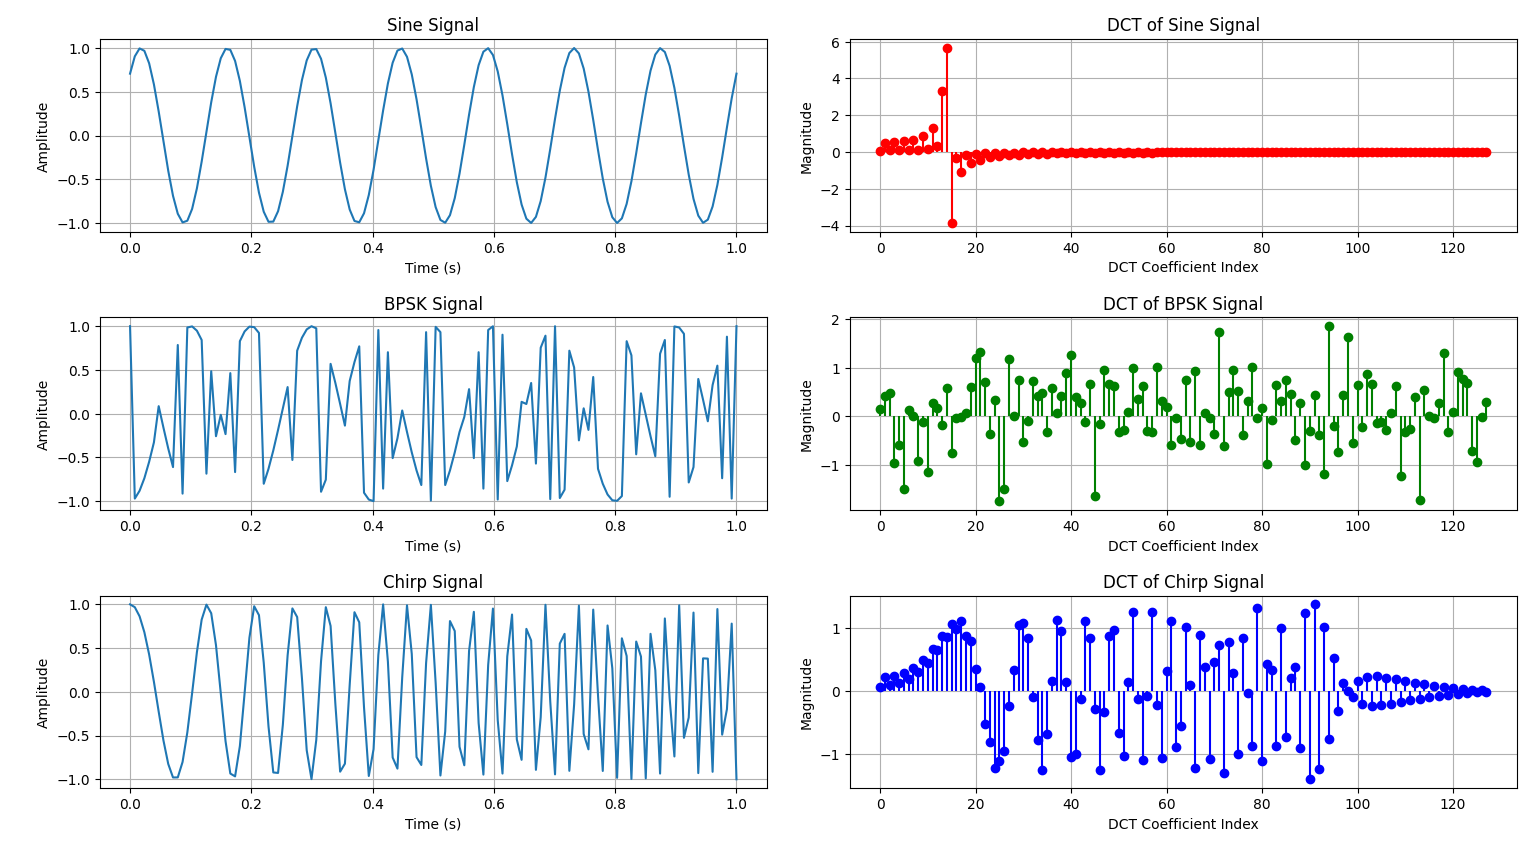
\includegraphics[width=1\linewidth,height=\textheight,keepaspectratio]{abar-cs_files/mediabag/input-dct.png}

}

\caption{DCT on different radar signals}

\end{figure}%

As shown above, other than the single tone sinusoids, the other two
matrices are not as sparse as expected. Even though, chirp signals are
expected to be not sparse, the BPSK signal is not sparse enough for
reconstruction.

So, for easy implementation of the dictionaries, the respective atoms
are created and is used as a dictionaries, that is, the bpsk and chirp
signal values are generated and filled to their respective matrix as
their dictionaries.

The mixer initially just added the 3 signals, but later on coefficients
were added for better understanding of its sparsity. The results,
however, are not really as satisfactory as expected. The signal
reconstruction is as shown

\begin{figure}[H]

{\centering \pandocbounded{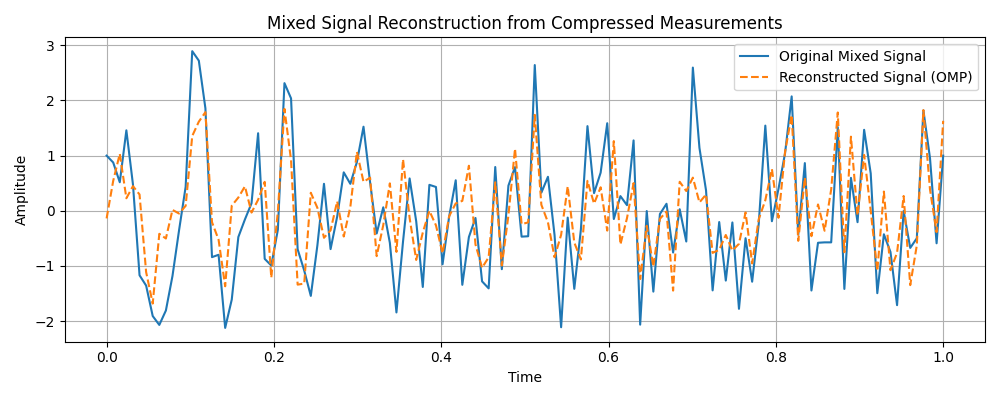
\includegraphics[keepaspectratio]{abar-cs_files/mediabag/n128-m64-ideal.png}}

}

\caption{Augmented Dictionary Implementation (Ideal): n=128 m=64}

\end{figure}%

\begin{figure}[H]

{\centering \pandocbounded{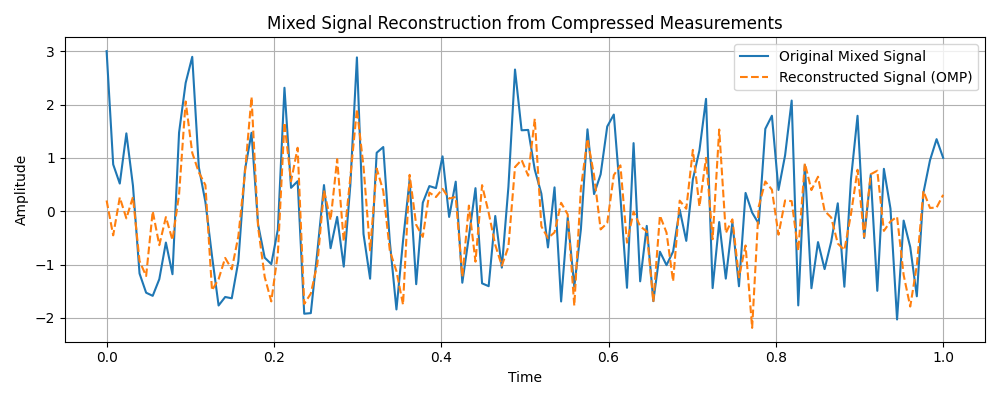
\includegraphics[keepaspectratio]{abar-cs_files/mediabag/n128-m64-noisy.png}}

}

\caption{Augmented Dictionary Implementation (Noisy): n=128 m=64}

\end{figure}%

so, now instead of just simply adding the signals as it is, coefficients
were added (a, b, c) such that each component of the input signal can be
tuned for observation.

\begin{figure}[H]

{\centering \pandocbounded{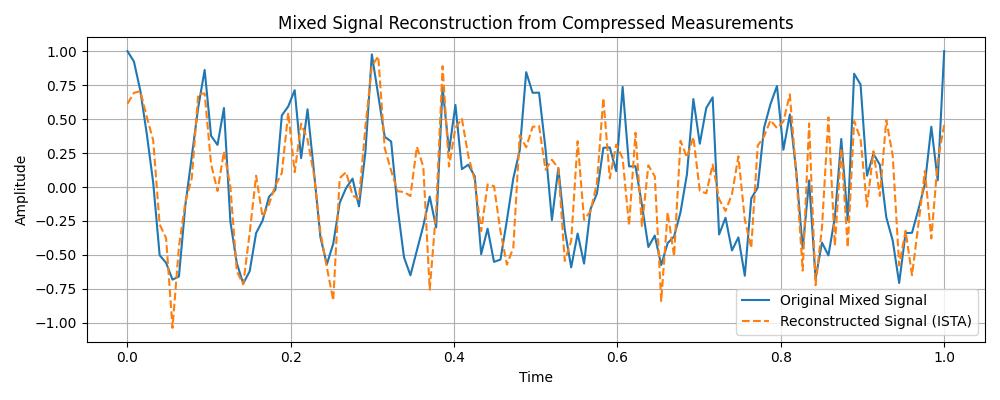
\includegraphics[keepaspectratio]{abar-cs_files/mediabag/n128-m64-ideal-mixer.png}}

}

\caption{Augmented Dictionary Implementation (Ideal) with mixer: n=128
m=64}

\end{figure}%

It is observed that the reconstruction error is pretty significant
compared to the overall amplitude of the input signal.

From the above implementation, we can say that the augmeneted dictionary
is a good attempt in assessing multiple radar input signals. But despite
that, the dictionary still needs to be pre-defined.

Moreover, most of the other radar signals are non-linear and some of
these signals can't have a basis for sparsity.

The best option is to adopt a learned method, or autoencoder to learn a
non-linear based basis for all the possible trained signals.

\newpage

\mainsection{CHAPTER 6: RECONSTRUCTION ALGORITHM UNROLLING}

\subsection{6.1 INTRODUCTION}\label{introduction-3}

As explained in the sections above, the current reconstruction
algorithms are iterative, hence require a long computational period
before an output is generated, which hampers the real time processing of
signal. One way to avoid this is improving the Reconstruction algorithms
to work real time.For such a case, machine learning techniques could
help. One promising approach is \textbf{algorithm unrolling} (also known
as unfolding), where the iterative steps of a reconstruction algorithm
are mapped onto the layers of a neural
network\autocite{fast-sparse-coding}. This technique enables the
integration of domain knowledge from classical algorithms with the
learning capacity of neural networks, resulting in models that are both
interpretable and highly effective.

Algorithm unrolling involves representing each iteration of an
algorithm---such as ISTA or OMP---as a layer in a neural network. The
parameters of these layers (e.g., thresholds, step sizes, or transforms)
can then be learned from data, allowing the network to adapt to the
specific characteristics of the signals and measurement process. This
approach not only accelerates convergence compared to traditional
iterative methods but also improves reconstruction quality, especially
in challenging scenarios with noise or model mismatch.

In this section, we discuss its advantages for real-time radar signal
processing, and introduce two unrolled algorithms - \textbf{Learned
ISTA(LISTA)} and \textbf{Learned CoD(LCoD)}.

\subsection{6.2 ADVANTAGES}\label{advantages}

Algorithm unfolding is a technique that transforms iterative algorithms
(like those used in optimization or signal processing) into a sequence
of layers, similar to neural networks. This approach offers several
advantages:

\textbf{Interpretability}: Each layer corresponds to a step in the
original algorithm, making the model's operations easier to understand
and analyze. \textbf{Efficiency}: By learning parameters for each layer,
unfolded algorithms can converge faster and require fewer iterations
than traditional methods. \textbf{Adaptability}: The unfolded structure
can be trained end-to-end, allowing it to adapt to specific data
distributions or tasks. \textbf{Performance}: Often achieves better
accuracy and robustness compared to standard iterative algorithms,
especially when combined with data-driven learning.

\subsection{6.3 LEARNED ISTA (LISTA)}\label{learned-ista-lista}

Learned ISTA (LISTA) is a neural network-based approach that unrolls the
traditional ISTA algorithm into a fixed number of layers, where each
layer mimics one iteration of ISTA. Unlike standard ISTA, where
parameters such as step size and thresholds are fixed, LISTA learns
these parameters from data during training. This enables faster
convergence and improved reconstruction accuracy. Each layer of the
LISTA network consists of a linear transformation followed by a
non-linear shrinkage (soft-thresholding) operation, and the parameters
of these operations are optimized by successive iterations. As a result,
LISTA combines the interpretability of classical algorithms with the
adaptability and efficiency of deep learning, making it well-suited for
real-time and large-scale compressed sensing applications.

\subsubsection{6.3.1 Algorithm
Implementation}\label{algorithm-implementation-2}

The algorithm implemented here has been improvised from the Python
implementation of LISTA from
\autocite{shlezinger_modelbaseddeeplearning}. All the required packages
were imported and the seed was fixed for reproducibility. A simulated
dataset was generated with a random dictionary and sparse signal. This
was plotted.

\begin{figure}[H]

{\centering \includegraphics[width=1\linewidth,height=\textheight,keepaspectratio]{abar-cs_files/mediabag/sample_seed.png}

}

\caption{Plot of Simulated Data}

\end{figure}%

First the ISTA algorithm was applied to the test set. The untrained
LISTA algorithm was then applied to the dataset, and the results were
compared with the standard ISTA algorithm. Now, the learned LISTA
algorithm was applied to the dataset, and the results were compared with
the standard ISTA algorithm.

\subsubsection{6.3.2 Observations and
Conclusion}\label{observations-and-conclusion}

The Iterations vs MSE plot of ISTA and Untrained LISTA shows clear
convergence. The untrained LISTA and classic ISTA algorithms should be
mathematically equivalent,but the starting point of both algorithms are
different, indicating issues with equivalence. But both algorithms
converge to the same reconstruction error.

\begin{figure}[H]

{\centering 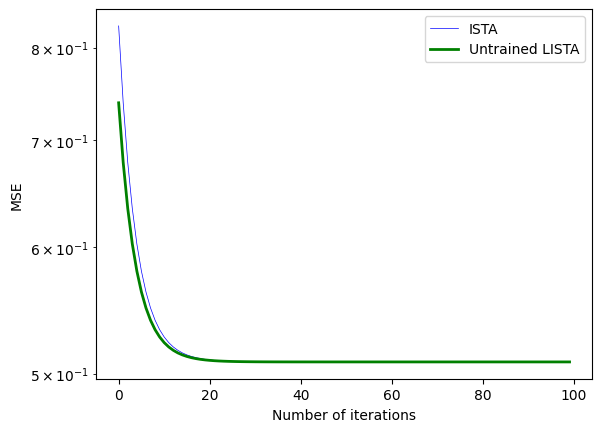
\includegraphics[width=1\linewidth,height=\textheight,keepaspectratio]{abar-cs_files/mediabag/ista_vs_untrained_li.png}

}

\caption{ISTA vs Untrained LISTA}

\end{figure}%

The iterations vs MSE plot of ISTA vs Trained LISTA is given below. The
trained LISTA algorithm converges to a better reconstruction error than
the untrained LISTA algorithm, using very low numbers of iterations. The
starting point of both algorithms is different, indicating the same
issues with equivalence as that of the above plot.

\begin{figure}[H]

{\centering \includegraphics[width=1\linewidth,height=\textheight,keepaspectratio]{abar-cs_files/mediabag/ista_vs_trained_list.png}

}

\caption{ISTA vs trained LISTA}

\end{figure}%

The conclusion is that Learned ISTA (LISTA) method is more than capable
of replacing ISTA, combining the interpretability of classic ISTA with
the adaptability and efficiency of neural networks.

\subsection{6.4 LEARNED COORDINATE DESCENT
(LCoD)}\label{learned-coordinate-descent-lcod}

The Learned Coordinate Descent (LCoD) algorithm is an optimization
technique that iteratively updates one coordinate (variable) at a time
to minimize a target function. Unlike standard coordinate descent, LCoD
leverages machine learning to adaptively select which coordinate to
update and how much to change it, based on patterns learned from data.
This approach can lead to faster convergence and improved performance,
especially in high-dimensional or structured problems.

\subsubsection{6.4.1 Algorithm
Implementation}\label{algorithm-implementation-3}

The code follows the same algorithmic flow as the previous Python
implementation of LISTA. All the required packages were imported and the
seed was fixed for reproducibility. A simulated dataset was generated
with a random dictionary and sparse signal.

\begin{figure}[H]

{\centering 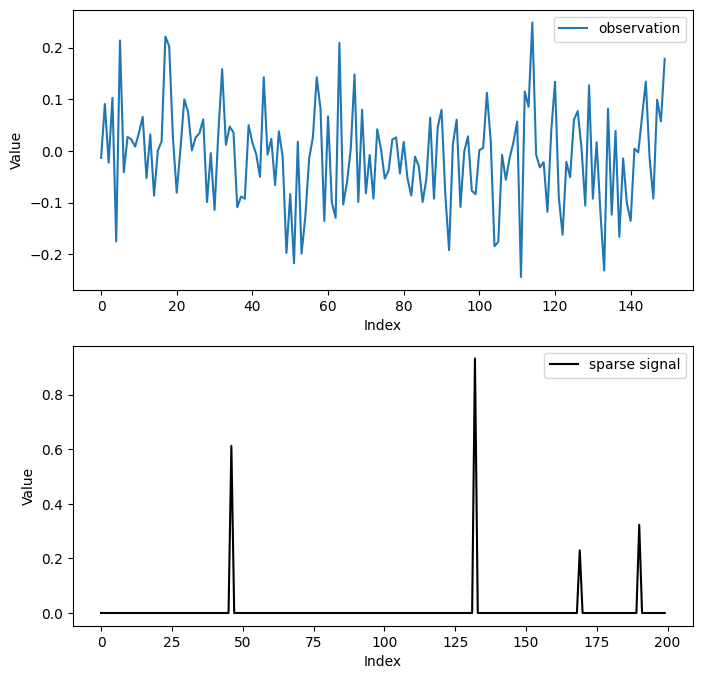
\includegraphics[width=1\linewidth,height=\textheight,keepaspectratio]{abar-cs_files/mediabag/sample_seed_cod.png}

}

\caption{Plot of Simulated Data}

\end{figure}%

First the CoD algorithm was applied to the test set. The untrained LCoD
algorithm was then applied to the dataset, and the results were compared
with the standard CoD algorithm. Now, the learned LCoD algorithm was
applied to the dataset, and the results were compared with the standard
CoD algorithm.

\subsubsection{6.4.2 Observations}\label{observations}

The Iterations vs MSE plot of CoD and Untrained LCoD shows that both
algorithms are mathematically equivalent. This is illustated in the plot
below. This is so, since no optimisations or changes were made to the
standard iterative step of CoD to create unrolled iterative step of
LCoD.

\begin{figure}[H]

{\centering 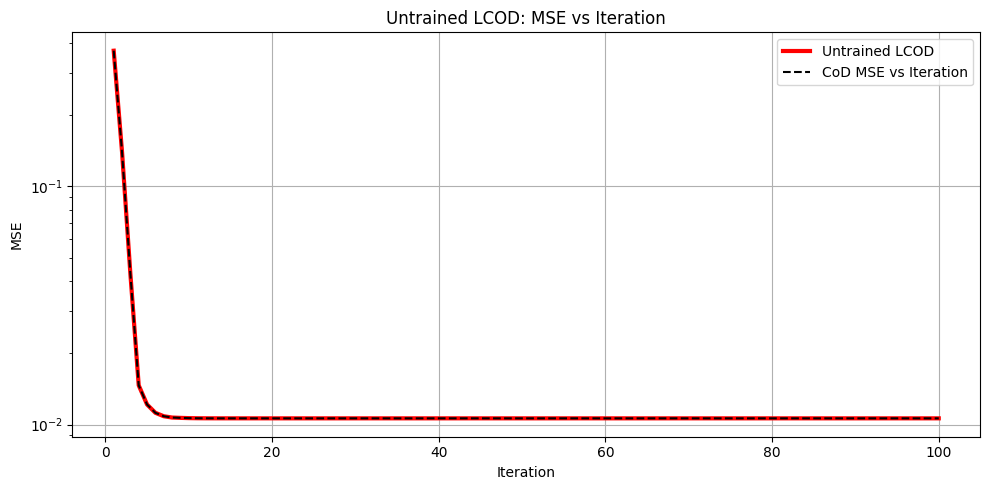
\includegraphics[width=1\linewidth,height=\textheight,keepaspectratio]{abar-cs_files/mediabag/CoDvsUntrainedCoD.png}

}

\caption{COD vs Untrained LCoD}

\end{figure}%

The iterations vs MSE plot of CoD vs Trained lCoD is given below. The
trained LISTA algorithm converges to a better reconstruction error than
the untrained LISTA algorithm, using lesser numbers of iterations.

\begin{figure}[H]

{\centering 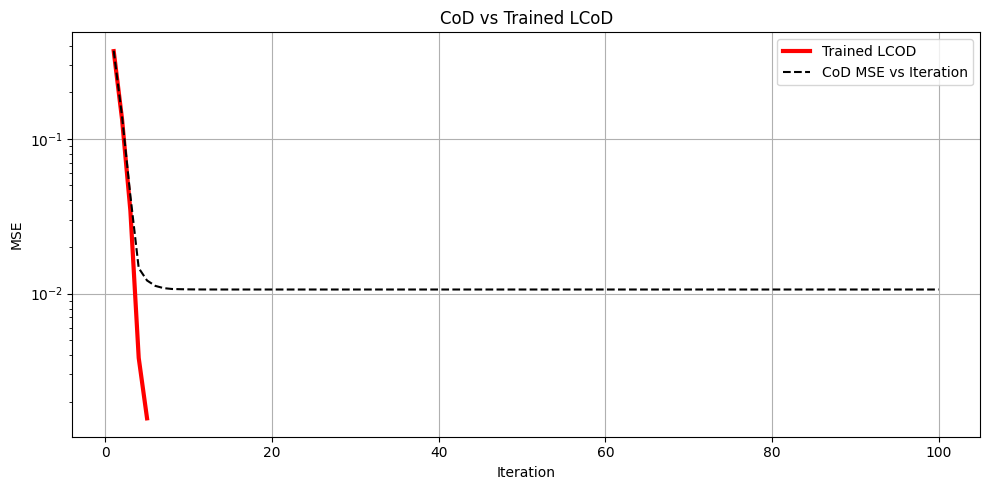
\includegraphics[width=1\linewidth,height=\textheight,keepaspectratio]{abar-cs_files/mediabag/CoDvsTrainedCoD.png}

}

\caption{COD vs trained LCoD}

\end{figure}%

A similar conclusion is made to the previous section.

\subsection{6.5 COMPARING BOTH
ALGORITHMS}\label{comparing-both-algorithms}

A Python implementation comparing the performance of Learned ISTA
(LISTA) and Learned CoD (LCoD) algorithms on a simulated dataset is
provided.

\begin{figure}[H]

{\centering 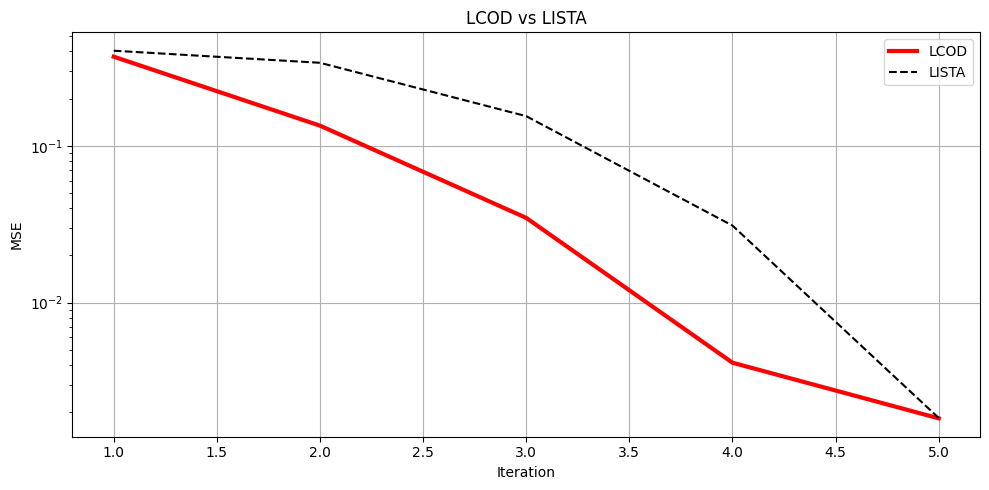
\includegraphics[width=1\linewidth,height=\textheight,keepaspectratio]{abar-cs_files/mediabag/lista_vs_lcod.png}

}

\caption{Comparison of LISTA and LCoD}

\end{figure}%

The plot above compares the MSE vs Iterations graph of Learned ISTA
(LISTA) and Learned CoD (LCoD) algorithms. Both algorithms converge to
the same reconstruction error. However, two major observations were
made:

\begin{enumerate}
\def\labelenumi{\arabic{enumi}.}
\tightlist
\item
  The iterations of LISTA is more inefficient compared to LCoD.
\end{enumerate}

This is because CoD is an iterative algorithm that selects and updates
one coordinate at a time greedily, hence it is guaranteed that there is
a change in MSE per iteration. ISTA does not have such guarantees, hence
LISTA may have higher MSE than LCoD at the same number of iterations.

\begin{enumerate}
\def\labelenumi{\arabic{enumi}.}
\setcounter{enumi}{1}
\tightlist
\item
  LCoD have higher computation time per iteration compared to LISTA.
\end{enumerate}

As explained above, CoD selects and updates coordinates one at a time
per iteration, hence it is more computationally expensive. Also, The
iterative step of CoD in the current implementation is not optimised for
torch operations, therefore steps involving torch operations take longer
to compute. The algorithm is serial by definition, thus training
involving batch operations needs workarounds to make it happen. Hence,
the current implementation takes longer time to compute than ISTA or
LISTA for the given problem.

The faster computation time of LISTA is beneficial for real-time signal
processing applications involving small-scale and parallelised
computing. But for larger scale LASSO problems, LCoD can be more
efficient, since the convergence guarentee of CoD means even though
individual iterations can be time-consuming, the number of iterations
required is much lower, which means the total computation time compared
to LISTA is less.

\subsection{6.6 FINAL REMARKS}\label{final-remarks}

The above observations show that Algorithm unrolling can significantly
improve the performance of iterative algorithms for a fraction of the
number of iterations. This method combines low sampling requirement of
compressed sensing algorithms with lower time complexity of learned ML
models, both of which are important requirements for real-time signal
processing applications.

\newpage

\mainsection{CHAPTER 7: FUTURE SCOPE}

This report lays a solid foundation for advanced research and practical
applications in compresses sensing for radar signal processing.

\begin{enumerate}
\def\labelenumi{\arabic{enumi}.}
\item
  In this project, the input signals are purely real, hence the use of
  DCT as basis. But in real life applications, the phase (complex) part
  is also applicable.
\item
  We have explored different reconstruction algorithms (like OMP, ISTA,
  CoD). The reconstruction can be further enhanced by other advanced
  algorithms like Fast ISTA (FISTA) or Alternating Direction Method of
  Multipliers (ADMM).
\item
  Instead of augmented dictionary, a learned dictionary (Autoencoder)
  can be used for predicting the non-linear radar signals.
\item
  Optimise torch operations for LCoD.
\item
  Trying to implement the real time processing into a hardware
  (FPGAs/Embedded GPUs) by reducing model size and complexity for low
  latency power.
\end{enumerate}

\newpage

\mainsection{REFERENCES}

\section{References}\label{references}

\printbibliography[heading=none]

\newpage

\mainsection{APPENDICES}

\textbf{FUNCTION:-}

\begin{itemize}
\tightlist
\item
  \textbf{Sine Wave Generator}
\end{itemize}

\begin{Shaded}
\begin{Highlighting}[]
\KeywordTok{def}\NormalTok{ generate\_sine\_signal(n, k, freq}\OperatorTok{=}\DecValTok{5}\NormalTok{, fs}\OperatorTok{=}\DecValTok{100}\NormalTok{):}
\NormalTok{    t }\OperatorTok{=}\NormalTok{ np.arange(n) }\OperatorTok{/}\NormalTok{ fs}
\NormalTok{    sum\_signal }\OperatorTok{=}\NormalTok{ np.zeros(n)}
    \ControlFlowTok{for}\NormalTok{ i }\KeywordTok{in} \BuiltInTok{range}\NormalTok{(}\DecValTok{1}\NormalTok{, k }\OperatorTok{+} \DecValTok{1}\NormalTok{):}
\NormalTok{        freq }\OperatorTok{=}\NormalTok{ i }\OperatorTok{*} \DecValTok{5}
\NormalTok{        sum\_signal }\OperatorTok{+=}\NormalTok{ np.sin(}\DecValTok{2} \OperatorTok{*}\NormalTok{ np.pi }\OperatorTok{*}\NormalTok{ freq }\OperatorTok{*}\NormalTok{ t)}
    \ControlFlowTok{return}\NormalTok{ sum\_signal}
\end{Highlighting}
\end{Shaded}

\begin{itemize}
\tightlist
\item
  \textbf{Noise Generator}
\end{itemize}

\begin{Shaded}
\begin{Highlighting}[]
\KeywordTok{def}\NormalTok{ add\_noise(y, snr\_db):}
\NormalTok{    signal\_power }\OperatorTok{=}\NormalTok{ np.mean(np.}\BuiltInTok{abs}\NormalTok{(y)}\OperatorTok{**}\DecValTok{2}\NormalTok{)}
\NormalTok{    snr\_linear }\OperatorTok{=} \DecValTok{10}\OperatorTok{**}\NormalTok{(snr\_db }\OperatorTok{/} \DecValTok{10}\NormalTok{)}
\NormalTok{    noise\_power }\OperatorTok{=}\NormalTok{ signal\_power }\OperatorTok{/}\NormalTok{ snr\_linear}
\NormalTok{    noise }\OperatorTok{=}\NormalTok{ np.sqrt(noise\_power) }\OperatorTok{*}\NormalTok{ np.random.randn(}\OperatorTok{*}\NormalTok{y.shape)}
    \ControlFlowTok{return}\NormalTok{ y }\OperatorTok{+}\NormalTok{ noise}
\end{Highlighting}
\end{Shaded}

\begin{itemize}
\tightlist
\item
  \textbf{OMP Function (Python)}
\end{itemize}

\begin{Shaded}
\begin{Highlighting}[]
\ImportTok{import}\NormalTok{ numpy }\ImportTok{as}\NormalTok{ np}

\KeywordTok{def}\NormalTok{ omp(y, A, tol}\OperatorTok{=}\FloatTok{1e{-}6}\NormalTok{):}
\NormalTok{    m, n }\OperatorTok{=}\NormalTok{ A.shape}
\NormalTok{    r }\OperatorTok{=}\NormalTok{ y.copy()}
\NormalTok{    idx\_set }\OperatorTok{=}\NormalTok{ []}
\NormalTok{    x\_hat }\OperatorTok{=}\NormalTok{ np.zeros(n)}

    \ControlFlowTok{for}\NormalTok{ \_ }\KeywordTok{in} \BuiltInTok{range}\NormalTok{(m):}
\NormalTok{        correlations }\OperatorTok{=}\NormalTok{ A.T }\OperatorTok{@}\NormalTok{ r}
\NormalTok{        idx }\OperatorTok{=}\NormalTok{ np.argmax(np.}\BuiltInTok{abs}\NormalTok{(correlations))}
\NormalTok{        idx\_set.append(idx)}
\NormalTok{        A\_selected }\OperatorTok{=}\NormalTok{ A[:, idx\_set]}
\NormalTok{        x\_ls, \_, \_, \_ }\OperatorTok{=}\NormalTok{ np.linalg.lstsq(A\_selected, y, rcond}\OperatorTok{=}\VariableTok{None}\NormalTok{)}
\NormalTok{        r }\OperatorTok{=}\NormalTok{ y }\OperatorTok{{-}}\NormalTok{ A\_selected }\OperatorTok{@}\NormalTok{ x\_ls}
        \ControlFlowTok{if}\NormalTok{ np.linalg.norm(r) }\OperatorTok{\textless{}}\NormalTok{ tol:}
            \ControlFlowTok{break}

\NormalTok{    x\_hat[idx\_set] }\OperatorTok{=}\NormalTok{ x\_ls}
    \ControlFlowTok{return}\NormalTok{ x\_hat}
\end{Highlighting}
\end{Shaded}

\begin{itemize}
\tightlist
\item
  \textbf{OMP Function (MATLAB)}
\end{itemize}

\begin{Shaded}
\begin{Highlighting}[]
\NormalTok{clc; close all; clear all;}
\NormalTok{function x = omp(A, b, K)}
\NormalTok{    originalA = A;               \% Store the original A}
\NormalTok{    norms = vecnorm(A);}
\NormalTok{    A = A ./ norms;}
\NormalTok{    r = b;}
\NormalTok{    Lambda = [];}
\NormalTok{    N = size(A, 2);}
\NormalTok{    x = zeros(N, 1);}

\NormalTok{    for k = 1:K}
\NormalTok{        h\_k = abs(A\textquotesingle{} * r);}
\NormalTok{        h\_k(Lambda) = 0;}
\NormalTok{        [\textasciitilde{}, l\_k] = max(h\_k);}

\NormalTok{        Lambda = [Lambda, l\_k];}
\NormalTok{        Asub = A(:, Lambda);}
\NormalTok{        x\_sub = Asub \textbackslash{} b;}

\NormalTok{        x = zeros(N, 1);}
\NormalTok{        x(Lambda) = x\_sub ./ norms(Lambda)\textquotesingle{};}
\NormalTok{        r = b {-} originalA(:, Lambda) * x(Lambda);   \% Corrected}
\NormalTok{    end}
\NormalTok{end}
\end{Highlighting}
\end{Shaded}

\begin{itemize}
\tightlist
\item
  \textbf{Monte-Carlo Trial}
\end{itemize}

\begin{Shaded}
\begin{Highlighting}[]
\ImportTok{import}\NormalTok{ numpy }\ImportTok{as}\NormalTok{ np}
\ImportTok{import}\NormalTok{ matplotlib.pyplot }\ImportTok{as}\NormalTok{ plt}
\ImportTok{from}\NormalTok{ scipy.fftpack }\ImportTok{import}\NormalTok{ dct, idct}
\ImportTok{from}\NormalTok{ numpy.linalg }\ImportTok{import}\NormalTok{ norm}

\KeywordTok{def}\NormalTok{ monte\_carlo\_trial(n, m, sampling\_rate):}
\NormalTok{    x\_time }\OperatorTok{=}\NormalTok{ generate\_sine\_signal(n, sampling\_rate)}
\NormalTok{    x\_sparse }\OperatorTok{=}\NormalTok{ dct(x\_time, norm}\OperatorTok{=}\StringTok{\textquotesingle{}ortho\textquotesingle{}}\NormalTok{)}
\NormalTok{    A }\OperatorTok{=}\NormalTok{ measurement(m, n)}
\NormalTok{    y }\OperatorTok{=}\NormalTok{ A }\OperatorTok{@}\NormalTok{ x\_sparse}
\NormalTok{    x\_sparse\_rec }\OperatorTok{=}\NormalTok{ omp(y, A)}
\NormalTok{    x\_time\_rec }\OperatorTok{=}\NormalTok{ idct(x\_sparse\_rec, norm}\OperatorTok{=}\StringTok{\textquotesingle{}ortho\textquotesingle{}}\NormalTok{)}
\NormalTok{    error }\OperatorTok{=}\NormalTok{ norm(x\_time }\OperatorTok{{-}}\NormalTok{ x\_time\_rec, }\BuiltInTok{ord}\OperatorTok{=}\DecValTok{2}\NormalTok{)}
    \ControlFlowTok{return}\NormalTok{ error}

\CommentTok{\# {-}{-}{-}{-} Monte Carlo Simulation and Plotting {-}{-}{-}{-}}
\NormalTok{num\_trials }\OperatorTok{=} \DecValTok{50}
\NormalTok{n\_values }\OperatorTok{=}\NormalTok{ [}\DecValTok{64}\NormalTok{, }\DecValTok{128}\NormalTok{, }\DecValTok{256}\NormalTok{]}
\NormalTok{m\_values }\OperatorTok{=}\NormalTok{ np.arange(}\DecValTok{2}\NormalTok{, }\DecValTok{65}\NormalTok{, }\DecValTok{2}\NormalTok{)  }\CommentTok{\# Number of measurements}
\NormalTok{noise\_val }\OperatorTok{=}\NormalTok{ np.arange(}\DecValTok{0}\NormalTok{, }\DecValTok{51}\NormalTok{, }\DecValTok{5}\NormalTok{)  }\CommentTok{\# Noise levels in dB}
\NormalTok{k\_values }\OperatorTok{=}\NormalTok{ np.arange(}\DecValTok{1}\NormalTok{, }\DecValTok{11}\NormalTok{, }\DecValTok{1}\NormalTok{)  }\CommentTok{\# Sparsity levels}
\NormalTok{sampling\_rate }\OperatorTok{=} \DecValTok{100}

\NormalTok{plt.figure(figsize}\OperatorTok{=}\NormalTok{(}\DecValTok{10}\NormalTok{, }\DecValTok{6}\NormalTok{))}

\ControlFlowTok{for}\NormalTok{ n }\KeywordTok{in}\NormalTok{ n\_values:}
\NormalTok{    avg\_errors }\OperatorTok{=}\NormalTok{ []}
    \ControlFlowTok{for}\NormalTok{ m }\KeywordTok{in}\NormalTok{ m\_values:}
        \ControlFlowTok{if}\NormalTok{ m }\OperatorTok{\textgreater{}=}\NormalTok{ n:}
\NormalTok{            avg\_errors.append(np.nan)}
            \ControlFlowTok{continue}
\NormalTok{        errors }\OperatorTok{=}\NormalTok{ []}
        \ControlFlowTok{for}\NormalTok{ \_ }\KeywordTok{in} \BuiltInTok{range}\NormalTok{(num\_trials):}
\NormalTok{            errors.append(monte\_carlo\_trial(n, m, sampling\_rate))}
\NormalTok{        avg\_errors.append(np.mean(errors))}
\NormalTok{    plt.plot(m\_values, avg\_errors, marker}\OperatorTok{=}\StringTok{\textquotesingle{}o\textquotesingle{}}\NormalTok{, label}\OperatorTok{=}\SpecialStringTok{f\textquotesingle{}n=}\SpecialCharTok{\{}\NormalTok{n}\SpecialCharTok{\}}\SpecialStringTok{\textquotesingle{}}\NormalTok{)}
\end{Highlighting}
\end{Shaded}

\begin{itemize}
\tightlist
\item
  \textbf{ISTA Function (Python)}
\end{itemize}

\begin{Shaded}
\begin{Highlighting}[]
\KeywordTok{def}\NormalTok{ soft\_thresholding(x, threshold):}
    \CommentTok{"""Soft thresholding operator h\_\{alpha/L\}"""}
    \ControlFlowTok{return}\NormalTok{ np.sign(x) }\OperatorTok{*}\NormalTok{ np.maximum(np.}\BuiltInTok{abs}\NormalTok{(x) }\OperatorTok{{-}}\NormalTok{ threshold, }\FloatTok{0.0}\NormalTok{)}

\KeywordTok{def}\NormalTok{ ista(X, W\_d, max\_iter}\OperatorTok{=}\DecValTok{200}\NormalTok{, tol}\OperatorTok{=}\FloatTok{1e{-}6}\NormalTok{):}
\NormalTok{    alpha }\OperatorTok{=} \FloatTok{0.1}
\NormalTok{    L }\OperatorTok{=} \FloatTok{1.1} \OperatorTok{*}\NormalTok{ np.linalg.norm(W\_d.T }\OperatorTok{@}\NormalTok{ W\_d, }\DecValTok{2}\NormalTok{)  }
    \CommentTok{\# L \textgreater{} max eigenvalue of W\_d.T @ W\_d}
\NormalTok{    m, n }\OperatorTok{=}\NormalTok{ W\_d.shape}
\NormalTok{    Z }\OperatorTok{=}\NormalTok{ np.zeros(n)}
    \ControlFlowTok{for}\NormalTok{ \_ }\KeywordTok{in} \BuiltInTok{range}\NormalTok{(max\_iter):}
\NormalTok{        Z\_old }\OperatorTok{=}\NormalTok{ Z.copy()}
\NormalTok{        gradient }\OperatorTok{=}\NormalTok{ W\_d.T }\OperatorTok{@}\NormalTok{ (W\_d }\OperatorTok{@}\NormalTok{ Z }\OperatorTok{{-}}\NormalTok{ X)}
\NormalTok{        Z }\OperatorTok{{-}=}\NormalTok{ gradient }\OperatorTok{/}\NormalTok{ L}
\NormalTok{        Z }\OperatorTok{=}\NormalTok{ soft\_thresholding(Z }\OperatorTok{{-}}\NormalTok{ (}\FloatTok{1.0} \OperatorTok{/}\NormalTok{ L) }\OperatorTok{*}\NormalTok{ gradient, alpha }\OperatorTok{/}\NormalTok{ L)}
        \ControlFlowTok{if}\NormalTok{ np.linalg.norm(Z }\OperatorTok{{-}}\NormalTok{ Z\_old, }\BuiltInTok{ord} \OperatorTok{=} \DecValTok{2}\NormalTok{) }\OperatorTok{\textless{}}\NormalTok{ tol:}
            \ControlFlowTok{break}
    \ControlFlowTok{return}\NormalTok{ Z}
\end{Highlighting}
\end{Shaded}

\begin{itemize}
\tightlist
\item
  \textbf{CoD Implementation (Python)}
\end{itemize}

\begin{Shaded}
\begin{Highlighting}[]
\CommentTok{\# Coordinate Descent Algorithm}
\NormalTok{z }\OperatorTok{=}\NormalTok{ np.zeros((n, }\DecValTok{1}\NormalTok{))}
\NormalTok{B }\OperatorTok{=}\NormalTok{ theta.T }\OperatorTok{@}\NormalTok{ y  }\CommentTok{\# Initial coefficients}
\NormalTok{S }\OperatorTok{=}\NormalTok{ np.eye(n) }\OperatorTok{{-}}\NormalTok{ theta.T }\OperatorTok{@}\NormalTok{ theta  }\CommentTok{\# Residual matrix}

\NormalTok{mse\_history }\OperatorTok{=}\NormalTok{ np.zeros(num\_iter)}

\ControlFlowTok{for}\NormalTok{ t }\KeywordTok{in} \BuiltInTok{range}\NormalTok{(num\_iter):}
\NormalTok{    z\_bar }\OperatorTok{=}\NormalTok{ np.sign(B) }\OperatorTok{*}\NormalTok{ np.maximum(np.}\BuiltInTok{abs}\NormalTok{(B) }\OperatorTok{{-}}\NormalTok{ alpha, }\DecValTok{0}\NormalTok{)}
\NormalTok{    k }\OperatorTok{=}\NormalTok{ np.argmax(np.}\BuiltInTok{abs}\NormalTok{(z }\OperatorTok{{-}}\NormalTok{ z\_bar))}
\NormalTok{    delta }\OperatorTok{=}\NormalTok{ z\_bar[k, }\DecValTok{0}\NormalTok{] }\OperatorTok{{-}}\NormalTok{ z[k, }\DecValTok{0}\NormalTok{]}
\NormalTok{    B }\OperatorTok{=}\NormalTok{ B }\OperatorTok{+}\NormalTok{ S[:, [k]] }\OperatorTok{*}\NormalTok{ delta}
\NormalTok{    z[k, }\DecValTok{0}\NormalTok{] }\OperatorTok{=}\NormalTok{ z\_bar[k, }\DecValTok{0}\NormalTok{]}
\NormalTok{    x\_rec\_iter }\OperatorTok{=}\NormalTok{ Psi }\OperatorTok{@}\NormalTok{ z}
\NormalTok{    mse\_history[t] }\OperatorTok{=}\NormalTok{ np.mean((x }\OperatorTok{{-}}\NormalTok{ x\_rec\_iter) }\OperatorTok{**} \DecValTok{2}\NormalTok{)}
\NormalTok{x\_rec }\OperatorTok{=}\NormalTok{ Psi }\OperatorTok{@}\NormalTok{ z}
\end{Highlighting}
\end{Shaded}

\begin{itemize}
\tightlist
\item
  \textbf{RADAR signal Generator}
\end{itemize}

\begin{Shaded}
\begin{Highlighting}[]
\ImportTok{import}\NormalTok{ numpy }\ImportTok{as}\NormalTok{ np}
\ImportTok{import}\NormalTok{ torch}
\ImportTok{from}\NormalTok{ scipy.signal }\ImportTok{import}\NormalTok{ chirp}

\KeywordTok{def}\NormalTok{ generate\_sine\_signals(batch\_size, length, freq\_range}\OperatorTok{=}\NormalTok{(}\DecValTok{1}\NormalTok{, }\DecValTok{10}\NormalTok{)):}
\NormalTok{    t }\OperatorTok{=}\NormalTok{ np.linspace(}\DecValTok{0}\NormalTok{, }\DecValTok{1}\NormalTok{, length)}
\NormalTok{    signals }\OperatorTok{=}\NormalTok{ []}
    \ControlFlowTok{for}\NormalTok{ \_ }\KeywordTok{in} \BuiltInTok{range}\NormalTok{(batch\_size):}
\NormalTok{        freq }\OperatorTok{=}\NormalTok{ np.random.uniform(}\OperatorTok{*}\NormalTok{freq\_range)}
\NormalTok{        phase }\OperatorTok{=}\NormalTok{ np.random.uniform(}\DecValTok{0}\NormalTok{, }\DecValTok{2}\OperatorTok{*}\NormalTok{np.pi)}
\NormalTok{        signal }\OperatorTok{=}\NormalTok{ np.sin(}\DecValTok{2} \OperatorTok{*}\NormalTok{ np.pi }\OperatorTok{*}\NormalTok{ freq }\OperatorTok{*}\NormalTok{ t }\OperatorTok{+}\NormalTok{ phase)}
\NormalTok{        signals.append(signal)}
    \ControlFlowTok{return}\NormalTok{ torch.tensor(signals, dtype}\OperatorTok{=}\NormalTok{torch.float32)}

\KeywordTok{def}\NormalTok{ generate\_bpsk\_signals(batch\_size, length):}
\NormalTok{    symbols }\OperatorTok{=} \DecValTok{2} \OperatorTok{*}\NormalTok{ torch.randint(}\DecValTok{0}\NormalTok{, }\DecValTok{2}\NormalTok{, (batch\_size, length)) }\OperatorTok{{-}} \DecValTok{1}
    \ControlFlowTok{return}\NormalTok{ symbols.}\BuiltInTok{float}\NormalTok{()}

\KeywordTok{def}\NormalTok{ generate\_chirp\_signals(batch\_size, length, f0}\OperatorTok{=}\DecValTok{5}\NormalTok{, f1}\OperatorTok{=}\DecValTok{50}\NormalTok{):}
\NormalTok{    t }\OperatorTok{=}\NormalTok{ np.linspace(}\DecValTok{0}\NormalTok{, }\DecValTok{1}\NormalTok{, length)}
\NormalTok{    signals }\OperatorTok{=}\NormalTok{ []}
    \ControlFlowTok{for}\NormalTok{ \_ }\KeywordTok{in} \BuiltInTok{range}\NormalTok{(batch\_size):}
\NormalTok{        signal }\OperatorTok{=}\NormalTok{ chirp(t, f0}\OperatorTok{=}\NormalTok{f0, f1}\OperatorTok{=}\NormalTok{f1, t1}\OperatorTok{=}\DecValTok{1}\NormalTok{, method}\OperatorTok{=}\StringTok{\textquotesingle{}linear\textquotesingle{}}\NormalTok{)}
\NormalTok{        signals.append(signal)}
    \ControlFlowTok{return}\NormalTok{ torch.tensor(signals, dtype}\OperatorTok{=}\NormalTok{torch.float32)}

\NormalTok{batch\_size }\OperatorTok{=} \DecValTok{1}
\NormalTok{length }\OperatorTok{=} \DecValTok{200}
\NormalTok{sine\_signals }\OperatorTok{=}\NormalTok{ generate\_sine\_signals(batch\_size, length)}
\NormalTok{bpsk\_signals }\OperatorTok{=}\NormalTok{ generate\_bpsk\_signals(batch\_size, length)}
\NormalTok{chirp\_signals }\OperatorTok{=}\NormalTok{ generate\_chirp\_signals(batch\_size, length)}
\end{Highlighting}
\end{Shaded}

\begin{itemize}
\tightlist
\item
  \textbf{Augmented Dictionary}
\end{itemize}

\begin{Shaded}
\begin{Highlighting}[]
\ImportTok{import}\NormalTok{ numpy }\ImportTok{as}\NormalTok{ np}
\ImportTok{from}\NormalTok{ scipy.fftpack }\ImportTok{import}\NormalTok{ dct, idct}
\ImportTok{import}\NormalTok{ matplotlib.pyplot }\ImportTok{as}\NormalTok{ plt}

\KeywordTok{def}\NormalTok{ soft\_thresholding(x, threshold):}
    \CommentTok{"""Soft thresholding operator h\_\{alpha/L\}"""}
    \ControlFlowTok{return}\NormalTok{ np.sign(x) }\OperatorTok{*}\NormalTok{ np.maximum(np.}\BuiltInTok{abs}\NormalTok{(x) }\OperatorTok{{-}}\NormalTok{ threshold, }\FloatTok{0.0}\NormalTok{)}

\KeywordTok{def}\NormalTok{ ista(X, W\_d, max\_iter}\OperatorTok{=}\DecValTok{200}\NormalTok{, tol}\OperatorTok{=}\FloatTok{1e{-}6}\NormalTok{):}
\NormalTok{    alpha }\OperatorTok{=} \FloatTok{0.1}
\NormalTok{    L }\OperatorTok{=} \FloatTok{1.1} \OperatorTok{*}\NormalTok{ np.linalg.norm(W\_d.T }\OperatorTok{@}\NormalTok{ W\_d, }\DecValTok{2}\NormalTok{)  }
    \CommentTok{\# L \textgreater{} max eigenvalue of W\_d.T @ W\_d}
\NormalTok{    m, n }\OperatorTok{=}\NormalTok{ W\_d.shape}
\NormalTok{    Z }\OperatorTok{=}\NormalTok{ np.zeros(n)}
    \ControlFlowTok{for}\NormalTok{ \_ }\KeywordTok{in} \BuiltInTok{range}\NormalTok{(max\_iter):}
\NormalTok{        Z\_old }\OperatorTok{=}\NormalTok{ Z.copy()}
\NormalTok{        gradient }\OperatorTok{=}\NormalTok{ W\_d.T }\OperatorTok{@}\NormalTok{ (W\_d }\OperatorTok{@}\NormalTok{ Z }\OperatorTok{{-}}\NormalTok{ X)}
\NormalTok{        Z }\OperatorTok{{-}=}\NormalTok{ gradient }\OperatorTok{/}\NormalTok{ L}
\NormalTok{        Z }\OperatorTok{=}\NormalTok{ soft\_thresholding(Z }\OperatorTok{{-}}\NormalTok{ (}\FloatTok{1.0} \OperatorTok{/}\NormalTok{ L) }\OperatorTok{*}\NormalTok{ gradient, alpha }\OperatorTok{/}\NormalTok{ L)}
        \ControlFlowTok{if}\NormalTok{ np.linalg.norm(Z }\OperatorTok{{-}}\NormalTok{ Z\_old, }\BuiltInTok{ord} \OperatorTok{=} \DecValTok{2}\NormalTok{) }\OperatorTok{\textless{}}\NormalTok{ tol:}
            \ControlFlowTok{break}
    \ControlFlowTok{return}\NormalTok{ Z}

\CommentTok{\# 1. Signal Setup}
\NormalTok{n }\OperatorTok{=} \BuiltInTok{int}\NormalTok{(}\BuiltInTok{input}\NormalTok{(}\StringTok{"Enter length of signal (n): "}\NormalTok{))  }\CommentTok{\# Signal length}
\NormalTok{t }\OperatorTok{=}\NormalTok{ np.linspace(}\DecValTok{0}\NormalTok{, }\DecValTok{1}\NormalTok{, n)}

\CommentTok{\# Sinusoidal component (tone)}
\NormalTok{tone }\OperatorTok{=}\NormalTok{ np.cos(}\DecValTok{2} \OperatorTok{*}\NormalTok{ np.pi }\OperatorTok{*} \DecValTok{10} \OperatorTok{*}\NormalTok{ t)}

\CommentTok{\# BPSK component}
\NormalTok{bits }\OperatorTok{=}\NormalTok{ np.random.randint(}\DecValTok{0}\NormalTok{, }\DecValTok{2}\NormalTok{, n)}
\NormalTok{bpsk }\OperatorTok{=}\NormalTok{ (}\DecValTok{2} \OperatorTok{*}\NormalTok{ bits }\OperatorTok{{-}} \DecValTok{1}\NormalTok{) }\OperatorTok{*}\NormalTok{ np.cos(}\DecValTok{2} \OperatorTok{*}\NormalTok{ np.pi }\OperatorTok{*} \DecValTok{5} \OperatorTok{*}\NormalTok{ t)}

\CommentTok{\# Chirp component}
\NormalTok{f0, k }\OperatorTok{=} \DecValTok{5}\NormalTok{, }\DecValTok{80}
\NormalTok{chirp }\OperatorTok{=}\NormalTok{ np.cos(}\DecValTok{2} \OperatorTok{*}\NormalTok{ np.pi }\OperatorTok{*}\NormalTok{ (f0 }\OperatorTok{*}\NormalTok{ t }\OperatorTok{+} \FloatTok{0.5} \OperatorTok{*}\NormalTok{ k }\OperatorTok{*}\NormalTok{ t}\OperatorTok{**}\DecValTok{2}\NormalTok{))}

\CommentTok{\# Mixed signal }
\NormalTok{a, b, c }\OperatorTok{=} \DecValTok{1}\NormalTok{, }\DecValTok{1}\NormalTok{, }\DecValTok{1}  \CommentTok{\# Coefficients for mixing}
\NormalTok{signal }\OperatorTok{=}\NormalTok{ a}\OperatorTok{*}\NormalTok{tone }\OperatorTok{+}\NormalTok{ b}\OperatorTok{*}\NormalTok{bpsk }\OperatorTok{+}\NormalTok{ c}\OperatorTok{*}\NormalTok{chirp}

\CommentTok{\# Sub{-}dictionary 1: DCT}
\NormalTok{D\_dct }\OperatorTok{=}\NormalTok{ np.eye(n)}
\NormalTok{D\_dct }\OperatorTok{=}\NormalTok{ idct(D\_dct, norm}\OperatorTok{=}\StringTok{\textquotesingle{}ortho\textquotesingle{}}\NormalTok{).T}

\CommentTok{\# Sub{-}dictionary 2: Chirp{-}like atoms}
\KeywordTok{def}\NormalTok{ generate\_chirp\_atoms(n, num\_atoms):}
\NormalTok{    t }\OperatorTok{=}\NormalTok{ np.linspace(}\DecValTok{0}\NormalTok{, }\DecValTok{1}\NormalTok{, n)}
\NormalTok{    D\_chirp }\OperatorTok{=}\NormalTok{ np.zeros((n, num\_atoms))}
    \ControlFlowTok{for}\NormalTok{ i }\KeywordTok{in} \BuiltInTok{range}\NormalTok{(num\_atoms):}
\NormalTok{        f0 }\OperatorTok{=}\NormalTok{ np.random.uniform(}\DecValTok{5}\NormalTok{, }\DecValTok{20}\NormalTok{)}
\NormalTok{        k }\OperatorTok{=}\NormalTok{ np.random.uniform(}\DecValTok{10}\NormalTok{, }\DecValTok{100}\NormalTok{)}
\NormalTok{        D\_chirp[:, i] }\OperatorTok{=}\NormalTok{ np.cos(}\DecValTok{2} \OperatorTok{*}\NormalTok{ np.pi }\OperatorTok{*}\NormalTok{ (f0 }\OperatorTok{*}\NormalTok{ t }\OperatorTok{+} \FloatTok{0.5} \OperatorTok{*}\NormalTok{ k }\OperatorTok{*}\NormalTok{ t}\OperatorTok{**}\DecValTok{2}\NormalTok{))}
\NormalTok{    D\_chirp }\OperatorTok{/=}\NormalTok{ np.linalg.norm(D\_chirp, axis}\OperatorTok{=}\DecValTok{0}\NormalTok{)}
    \ControlFlowTok{return}\NormalTok{ D\_chirp}

\NormalTok{D\_chirp }\OperatorTok{=}\NormalTok{ generate\_chirp\_atoms(n, n)}

\CommentTok{\# Sub{-}dictionary 3: BPSK atoms}
\KeywordTok{def}\NormalTok{ generate\_bpsk\_atoms(n, num\_atoms, fc}\OperatorTok{=}\DecValTok{5}\NormalTok{, fs}\OperatorTok{=}\DecValTok{100}\NormalTok{):}
\NormalTok{    t }\OperatorTok{=}\NormalTok{ np.arange(n) }\OperatorTok{/}\NormalTok{ fs}
\NormalTok{    D\_bpsk }\OperatorTok{=}\NormalTok{ np.zeros((n, num\_atoms))}
    \ControlFlowTok{for}\NormalTok{ i }\KeywordTok{in} \BuiltInTok{range}\NormalTok{(num\_atoms):}
\NormalTok{        bits }\OperatorTok{=}\NormalTok{ np.random.randint(}\DecValTok{0}\NormalTok{, }\DecValTok{2}\NormalTok{, n)}
\NormalTok{        symbols }\OperatorTok{=} \DecValTok{2} \OperatorTok{*}\NormalTok{ bits }\OperatorTok{{-}} \DecValTok{1}
\NormalTok{        D\_bpsk[:, i] }\OperatorTok{=}\NormalTok{ symbols }\OperatorTok{*}\NormalTok{ np.cos(}\DecValTok{2} \OperatorTok{*}\NormalTok{ np.pi }\OperatorTok{*}\NormalTok{ fc }\OperatorTok{*}\NormalTok{ t)}
    \CommentTok{\# Normalize atoms}
\NormalTok{    D\_bpsk }\OperatorTok{/=}\NormalTok{ np.linalg.norm(D\_bpsk, axis}\OperatorTok{=}\DecValTok{0}\NormalTok{)}
    \ControlFlowTok{return}\NormalTok{ D\_bpsk}

\CommentTok{\# Usage:}
\NormalTok{D\_bpsk }\OperatorTok{=}\NormalTok{ generate\_bpsk\_atoms(n, n)}
\NormalTok{D\_total }\OperatorTok{=}\NormalTok{ np.concatenate([D\_dct, D\_dct, D\_chirp], axis}\OperatorTok{=}\DecValTok{1}\NormalTok{)}

\CommentTok{\# Compressed Measurement}
\NormalTok{m }\OperatorTok{=} \BuiltInTok{int}\NormalTok{(}\BuiltInTok{input}\NormalTok{(}\StringTok{"Enter number of compressed samples (m \textless{} n): "}\NormalTok{))  }\CommentTok{\# Compressed samples}
\NormalTok{Phi }\OperatorTok{=}\NormalTok{ np.random.randn(m, n)}\CommentTok{\# / np.sqrt(k)  \# Measurement matrix}
\NormalTok{y }\OperatorTok{=}\NormalTok{ Phi }\OperatorTok{@}\NormalTok{ signal}

\CommentTok{\# Add noise to the measurements}
\NormalTok{snr\_db }\OperatorTok{=} \BuiltInTok{int}\NormalTok{(}\BuiltInTok{input}\NormalTok{(}\StringTok{"Enter noise to be added (dB): "}\NormalTok{))  }\CommentTok{\# Signal{-}to{-}noise ratio in dB}
\NormalTok{y\_noisy }\OperatorTok{=}\NormalTok{ add\_noise(y, snr\_db)}

\CommentTok{\# Construct sensing matrix (Theta)}
\NormalTok{A }\OperatorTok{=}\NormalTok{ Phi }\OperatorTok{@}\NormalTok{ D\_total}

\CommentTok{\# Sparse Recovery using ISTA}
\CommentTok{\#z = ista(y\_noisy, A)}
\NormalTok{z }\OperatorTok{=}\NormalTok{ omp(y, A)}
\NormalTok{signal\_hat }\OperatorTok{=}\NormalTok{ D\_total }\OperatorTok{@}\NormalTok{ z}

\CommentTok{\# Calculate reconstruction error}
\NormalTok{error }\OperatorTok{=}\NormalTok{ np.linalg.norm(signal }\OperatorTok{{-}}\NormalTok{ signal\_hat)}
\BuiltInTok{print}\NormalTok{(}\SpecialStringTok{f"Reconstruction error (L2 norm): }\SpecialCharTok{\{}\NormalTok{error}\SpecialCharTok{:.4f\}}\SpecialStringTok{"}\NormalTok{)}

\CommentTok{\# 9. Plot original and reconstructed}
\NormalTok{plt.figure(figsize}\OperatorTok{=}\NormalTok{(}\DecValTok{10}\NormalTok{, }\DecValTok{4}\NormalTok{))}
\NormalTok{plt.plot(t, signal, label}\OperatorTok{=}\StringTok{"Original Mixed Signal"}\NormalTok{)}
\NormalTok{plt.plot(t, signal\_hat, }\StringTok{\textquotesingle{}{-}{-}\textquotesingle{}}\NormalTok{, label}\OperatorTok{=}\StringTok{"Reconstructed Signal (ISTA)"}\NormalTok{)}
\NormalTok{plt.title(}\StringTok{"Mixed Signal Reconstruction from Compressed Measurements"}\NormalTok{)}
\NormalTok{plt.xlabel(}\StringTok{"Time"}\NormalTok{)}
\NormalTok{plt.ylabel(}\StringTok{"Amplitude"}\NormalTok{)}
\NormalTok{plt.legend()}
\NormalTok{plt.grid(}\VariableTok{True}\NormalTok{)}
\NormalTok{plt.tight\_layout()}
\NormalTok{plt.show()}
\end{Highlighting}
\end{Shaded}

\begin{itemize}
\tightlist
\item
  \textbf{Creating Simulated Dataset}
\end{itemize}

\begin{Shaded}
\begin{Highlighting}[]
\KeywordTok{class}\NormalTok{ SimulatedData(Data.Dataset): }\CommentTok{\#Creates tuple (x, H, s) for each sample}
    \KeywordTok{def} \FunctionTok{\_\_init\_\_}\NormalTok{(}\VariableTok{self}\NormalTok{, x, H, s):}
        \VariableTok{self}\NormalTok{.x }\OperatorTok{=}\NormalTok{ x}
        \VariableTok{self}\NormalTok{.s }\OperatorTok{=}\NormalTok{ s}
        \VariableTok{self}\NormalTok{.H }\OperatorTok{=}\NormalTok{ H}

    \KeywordTok{def} \FunctionTok{\_\_len\_\_}\NormalTok{(}\VariableTok{self}\NormalTok{):}
        \ControlFlowTok{return} \VariableTok{self}\NormalTok{.x.shape[}\DecValTok{0}\NormalTok{]}

    \KeywordTok{def} \FunctionTok{\_\_getitem\_\_}\NormalTok{(}\VariableTok{self}\NormalTok{, idx):}
\NormalTok{        x }\OperatorTok{=} \VariableTok{self}\NormalTok{.x[idx, :]}
\NormalTok{        H }\OperatorTok{=} \VariableTok{self}\NormalTok{.H}
\NormalTok{        s }\OperatorTok{=} \VariableTok{self}\NormalTok{.s[idx, :]}
        \ControlFlowTok{return}\NormalTok{ x, H, s}

\KeywordTok{def}\NormalTok{ create\_data\_set(H, n, m, k, N}\OperatorTok{=}\DecValTok{1000}\NormalTok{, batch\_size}\OperatorTok{=}\DecValTok{512}\NormalTok{, signal\_dev}\OperatorTok{=}\FloatTok{0.5}\NormalTok{, noise\_dev}\OperatorTok{=}\FloatTok{0.01}\NormalTok{): }\CommentTok{\#function to create dataset}
    \CommentTok{\# Initialization}
\NormalTok{    x }\OperatorTok{=}\NormalTok{ torch.zeros(N, n)}
\NormalTok{    s }\OperatorTok{=}\NormalTok{ torch.zeros(N, m)}

    \CommentTok{\# Create signals}
    \ControlFlowTok{for}\NormalTok{ i }\KeywordTok{in} \BuiltInTok{range}\NormalTok{(N):}
        \CommentTok{\# Create a k{-}sparsed signal s}
\NormalTok{        index\_k }\OperatorTok{=}\NormalTok{ np.random.choice(m, k, replace}\OperatorTok{=}\VariableTok{False}\NormalTok{)}
\NormalTok{        peaks }\OperatorTok{=}\NormalTok{ signal\_dev }\OperatorTok{*}\NormalTok{ np.random.randn(k)}

\NormalTok{        s[i, index\_k] }\OperatorTok{=}\NormalTok{ torch.from\_numpy(peaks).to(s)}

        \CommentTok{\# X = Hs+w}
\NormalTok{        x[i, :] }\OperatorTok{=}\NormalTok{ H }\OperatorTok{@}\NormalTok{ s[i, :] }\OperatorTok{+}\NormalTok{ noise\_dev }\OperatorTok{*}\NormalTok{ torch.randn(n)}

\NormalTok{    simulated }\OperatorTok{=}\NormalTok{ SimulatedData(x}\OperatorTok{=}\NormalTok{x, H}\OperatorTok{=}\NormalTok{H, s}\OperatorTok{=}\NormalTok{s)}
\NormalTok{    data\_loader }\OperatorTok{=}\NormalTok{ Data.DataLoader(dataset}\OperatorTok{=}\NormalTok{simulated, batch\_size}\OperatorTok{=}\NormalTok{batch\_size, shuffle}\OperatorTok{=}\VariableTok{True}\NormalTok{)}
    \ControlFlowTok{return}\NormalTok{ data\_loader}

\NormalTok{N }\OperatorTok{=} \DecValTok{1000} \CommentTok{\# number of samples}
\NormalTok{n }\OperatorTok{=} \DecValTok{150} \CommentTok{\# dim(x)}
\NormalTok{m }\OperatorTok{=} \DecValTok{200} \CommentTok{\# dim(s)}
\NormalTok{k }\OperatorTok{=} \DecValTok{4} \CommentTok{\# k{-}sparse signal}
\NormalTok{T\_t }\OperatorTok{=} \DecValTok{5}  \CommentTok{\# Number of iterations}

\CommentTok{\# Measurement matrix}
\NormalTok{H }\OperatorTok{=}\NormalTok{ torch.randn(n, m)}
\NormalTok{H }\OperatorTok{/=}\NormalTok{ torch.norm(H, dim}\OperatorTok{=}\DecValTok{0}\NormalTok{)}

\CommentTok{\# Generate datasets}
\NormalTok{train\_loader }\OperatorTok{=}\NormalTok{ create\_data\_set(H, n}\OperatorTok{=}\NormalTok{n, m}\OperatorTok{=}\NormalTok{m, k}\OperatorTok{=}\NormalTok{k, N}\OperatorTok{=}\NormalTok{N)}
\NormalTok{test\_loader }\OperatorTok{=}\NormalTok{ create\_data\_set(H, n}\OperatorTok{=}\NormalTok{n, m}\OperatorTok{=}\NormalTok{m, k}\OperatorTok{=}\NormalTok{k, N}\OperatorTok{=}\NormalTok{N, batch\_size}\OperatorTok{=}\NormalTok{N)}
\end{Highlighting}
\end{Shaded}

\begin{itemize}
\tightlist
\item
  \textbf{LISTA Class}
\end{itemize}

\begin{Shaded}
\begin{Highlighting}[]
\KeywordTok{class}\NormalTok{ LISTA\_Model(nn.Module):}
    \KeywordTok{def} \FunctionTok{\_\_init\_\_}\NormalTok{(}\VariableTok{self}\NormalTok{, n, m, L, T}\OperatorTok{=}\DecValTok{6}\NormalTok{, rho}\OperatorTok{=}\FloatTok{1.0}\NormalTok{, H}\OperatorTok{=}\VariableTok{None}\NormalTok{):}
        \BuiltInTok{super}\NormalTok{(LISTA\_Model, }\VariableTok{self}\NormalTok{).}\FunctionTok{\_\_init\_\_}\NormalTok{()}
        \VariableTok{self}\NormalTok{.n, }\VariableTok{self}\NormalTok{.m }\OperatorTok{=}\NormalTok{ n, m}
        \VariableTok{self}\NormalTok{.H }\OperatorTok{=}\NormalTok{ H}
        \VariableTok{self}\NormalTok{.L }\OperatorTok{=}\NormalTok{ L}
        \VariableTok{self}\NormalTok{.T }\OperatorTok{=}\NormalTok{ T  }\CommentTok{\# ISTA Iterations}
        \VariableTok{self}\NormalTok{.rho }\OperatorTok{=}\NormalTok{ rho  }\CommentTok{\# Lagrangian Multiplier}
        \VariableTok{self}\NormalTok{.A }\OperatorTok{=}\NormalTok{ nn.Linear(n, m, bias}\OperatorTok{=}\VariableTok{False}\NormalTok{)  }\CommentTok{\# Weight Matrix}
        \VariableTok{self}\NormalTok{.B }\OperatorTok{=}\NormalTok{ nn.Linear(m, m, bias}\OperatorTok{=}\VariableTok{False}\NormalTok{)  }\CommentTok{\# Weight Matrix}
        \CommentTok{\# ISTA Stepsizes eta}
        \VariableTok{self}\NormalTok{.beta }\OperatorTok{=}\NormalTok{ nn.Parameter(torch.ones(T }\OperatorTok{+} \DecValTok{1}\NormalTok{, }\DecValTok{1}\NormalTok{, }\DecValTok{1}\NormalTok{)}\OperatorTok{/}\NormalTok{L, requires\_grad}\OperatorTok{=}\VariableTok{True}\NormalTok{)}
        \VariableTok{self}\NormalTok{.mu }\OperatorTok{=}\NormalTok{ nn.Parameter(torch.ones(T }\OperatorTok{+} \DecValTok{1}\NormalTok{, }\DecValTok{1}\NormalTok{, }\DecValTok{1}\NormalTok{)}\OperatorTok{/}\NormalTok{L, requires\_grad}\OperatorTok{=}\VariableTok{True}\NormalTok{)}
        \CommentTok{\# Initialization}
        \ControlFlowTok{if}\NormalTok{ H }\KeywordTok{is} \KeywordTok{not} \VariableTok{None}\NormalTok{:}
            \VariableTok{self}\NormalTok{.A.weight.data }\OperatorTok{=}\NormalTok{ H.t()}
            \VariableTok{self}\NormalTok{.B.weight.data }\OperatorTok{=}\NormalTok{ H.t() }\OperatorTok{@}\NormalTok{ H}

        \CommentTok{\textquotesingle{}\textquotesingle{}\textquotesingle{}for param in self.A.parameters(): \# A needs no\_grad (should not be trained)}
\CommentTok{            param.requires\_grad = False}
\CommentTok{        for param in self.B.parameters():\# B needs no\_grad (should not be trained)}
\CommentTok{            param.requires\_grad = False\textquotesingle{}\textquotesingle{}\textquotesingle{}}
       
    \KeywordTok{def}\NormalTok{ \_shrink(}\VariableTok{self}\NormalTok{, s, beta):}
        \ControlFlowTok{return}\NormalTok{ beta }\OperatorTok{*}\NormalTok{ F.softshrink(s }\OperatorTok{/}\NormalTok{ beta, lambd}\OperatorTok{=}\VariableTok{self}\NormalTok{.rho)}

    \KeywordTok{def}\NormalTok{ forward(}\VariableTok{self}\NormalTok{, x, s\_gt}\OperatorTok{=}\VariableTok{None}\NormalTok{):}
\NormalTok{        mse\_vs\_itr }\OperatorTok{=}\NormalTok{ []}

\NormalTok{        s\_hat }\OperatorTok{=} \VariableTok{self}\NormalTok{.\_shrink(}\VariableTok{self}\NormalTok{.mu[}\DecValTok{0}\NormalTok{, :, :] }\OperatorTok{*} \VariableTok{self}\NormalTok{.A(x), }\VariableTok{self}\NormalTok{.beta[}\DecValTok{0}\NormalTok{, :, :])}
        \ControlFlowTok{for}\NormalTok{ i }\KeywordTok{in} \BuiltInTok{range}\NormalTok{(}\DecValTok{1}\NormalTok{, }\VariableTok{self}\NormalTok{.T }\OperatorTok{+} \DecValTok{1}\NormalTok{):}
\NormalTok{            s\_hat }\OperatorTok{=} \VariableTok{self}\NormalTok{.\_shrink(s\_hat }\OperatorTok{{-}} \VariableTok{self}\NormalTok{.mu[i, :, :] }\OperatorTok{*} \VariableTok{self}\NormalTok{.B(s\_hat) }\OperatorTok{+} \VariableTok{self}\NormalTok{.mu[i, :, :] }\OperatorTok{*} \VariableTok{self}\NormalTok{.A(x),}
                                 \VariableTok{self}\NormalTok{.beta[i, :, :], )}
            
            \CommentTok{\# Aggregate each iteration\textquotesingle{}s MSE loss}
            \ControlFlowTok{if}\NormalTok{ s\_gt }\KeywordTok{is} \KeywordTok{not} \VariableTok{None}\NormalTok{:}
\NormalTok{                mse\_vs\_itr.append(F.mse\_loss(s\_hat.detach(), s\_gt.detach(), reduction}\OperatorTok{=}\StringTok{"sum"}\NormalTok{).data.item())}

        \ControlFlowTok{return}\NormalTok{ s\_hat, mse\_vs\_itr}
\end{Highlighting}
\end{Shaded}

\begin{itemize}
\tightlist
\item
  \textbf{LCoD Class}
\end{itemize}

\begin{Shaded}
\begin{Highlighting}[]
\KeywordTok{class}\NormalTok{ LearnedCoD(nn.Module):}
    \KeywordTok{def} \FunctionTok{\_\_init\_\_}\NormalTok{(}\VariableTok{self}\NormalTok{, H, T}\OperatorTok{=}\DecValTok{10}\NormalTok{, learn\_alpha}\OperatorTok{=}\VariableTok{True}\NormalTok{):}
        \BuiltInTok{super}\NormalTok{(LearnedCoD, }\VariableTok{self}\NormalTok{).}\FunctionTok{\_\_init\_\_}\NormalTok{()}
        \VariableTok{self}\NormalTok{.T }\OperatorTok{=}\NormalTok{ T}
        \VariableTok{self}\NormalTok{.H }\OperatorTok{=}\NormalTok{ H}
        \VariableTok{self}\NormalTok{.m }\OperatorTok{=}\NormalTok{ H.shape[}\DecValTok{1}\NormalTok{]}

        \CommentTok{\# Fixed matrices (you can make them learnable if needed)}
        \VariableTok{self}\NormalTok{.B\_mat }\OperatorTok{=}\NormalTok{ nn.Parameter(H.T.clone(), requires\_grad}\OperatorTok{=}\VariableTok{False}\NormalTok{)}
        \VariableTok{self}\NormalTok{.S\_mat }\OperatorTok{=}\NormalTok{ nn.Parameter(torch.eye(}\VariableTok{self}\NormalTok{.m, dtype}\OperatorTok{=}\NormalTok{torch.float64) }\OperatorTok{{-}}\NormalTok{ H.T }\OperatorTok{@}\NormalTok{ H, requires\_grad}\OperatorTok{=}\VariableTok{False}\NormalTok{)}

        \CommentTok{\# Learnable thresholds}
        \ControlFlowTok{if}\NormalTok{ learn\_alpha:}
            \VariableTok{self}\NormalTok{.alpha\_list }\OperatorTok{=}\NormalTok{ nn.ParameterList([nn.Parameter(torch.tensor(}\FloatTok{0.05}\NormalTok{, dtype}\OperatorTok{=}\NormalTok{torch.float64)) }\ControlFlowTok{for}\NormalTok{ \_ }\KeywordTok{in} \BuiltInTok{range}\NormalTok{(T)])}
        \ControlFlowTok{else}\NormalTok{:}
            \VariableTok{self}\NormalTok{.alpha\_list }\OperatorTok{=}\NormalTok{ [torch.tensor(}\FloatTok{0.05}\NormalTok{, dtype}\OperatorTok{=}\NormalTok{torch.float64) }\ControlFlowTok{for}\NormalTok{ \_ }\KeywordTok{in} \BuiltInTok{range}\NormalTok{(T)]}

    \KeywordTok{def}\NormalTok{ soft\_threshold(}\VariableTok{self}\NormalTok{, B, alpha):}
        \ControlFlowTok{return}\NormalTok{ torch.sign(B) }\OperatorTok{*}\NormalTok{ torch.maximum(torch.}\BuiltInTok{abs}\NormalTok{(B) }\OperatorTok{{-}}\NormalTok{ alpha, torch.zeros\_like(B))}

    \KeywordTok{def}\NormalTok{ forward(}\VariableTok{self}\NormalTok{, x, s\_gt}\OperatorTok{=}\VariableTok{None}\NormalTok{):}
        \ControlFlowTok{if}\NormalTok{ x.dim() }\OperatorTok{==} \DecValTok{2} \KeywordTok{and}\NormalTok{ x.shape[}\DecValTok{1}\NormalTok{] }\OperatorTok{==} \VariableTok{self}\NormalTok{.H.shape[}\DecValTok{0}\NormalTok{]:}
\NormalTok{            batch\_size }\OperatorTok{=}\NormalTok{ x.shape[}\DecValTok{0}\NormalTok{]}
\NormalTok{            z\_out }\OperatorTok{=}\NormalTok{ []}
\NormalTok{            mse\_list }\OperatorTok{=}\NormalTok{ []}

            \ControlFlowTok{for}\NormalTok{ i }\KeywordTok{in} \BuiltInTok{range}\NormalTok{(batch\_size):}
\NormalTok{                z\_i, mse\_i }\OperatorTok{=} \VariableTok{self}\NormalTok{.forward(x[i].unsqueeze(}\DecValTok{1}\NormalTok{), s\_gt[i].unsqueeze(}\DecValTok{1}\NormalTok{) }\ControlFlowTok{if}\NormalTok{ s\_gt }\KeywordTok{is} \KeywordTok{not} \VariableTok{None} \ControlFlowTok{else} \VariableTok{None}\NormalTok{)}
\NormalTok{                z\_out.append(z\_i.squeeze(}\DecValTok{1}\NormalTok{))  }\CommentTok{\# (m, 1) {-}\textgreater{} (m,)}
                \ControlFlowTok{if}\NormalTok{ s\_gt }\KeywordTok{is} \KeywordTok{not} \VariableTok{None}\NormalTok{:}
\NormalTok{                    mse\_list.append(mse\_i)}

\NormalTok{            z\_out }\OperatorTok{=}\NormalTok{ torch.stack(z\_out, dim}\OperatorTok{=}\DecValTok{0}\NormalTok{)  }\CommentTok{\# shape: (batch\_size, m)}
            \ControlFlowTok{if}\NormalTok{ s\_gt }\KeywordTok{is} \KeywordTok{not} \VariableTok{None}\NormalTok{:}
\NormalTok{                mse\_avg }\OperatorTok{=}\NormalTok{ torch.stack(mse\_list, dim}\OperatorTok{=}\DecValTok{0}\NormalTok{).mean(dim}\OperatorTok{=}\DecValTok{0}\NormalTok{)}
                \ControlFlowTok{return}\NormalTok{ z\_out, mse\_avg}
            \ControlFlowTok{else}\NormalTok{:}
                \ControlFlowTok{return}\NormalTok{ z\_out, }\VariableTok{None}

    \CommentTok{\# Single sample mode (x shape = [n, 1])}
\NormalTok{        B }\OperatorTok{=} \VariableTok{self}\NormalTok{.B\_mat }\OperatorTok{@}\NormalTok{ x  }\CommentTok{\# shape: (m, 1)}
\NormalTok{        z }\OperatorTok{=}\NormalTok{ torch.zeros((}\VariableTok{self}\NormalTok{.m, }\DecValTok{1}\NormalTok{), dtype}\OperatorTok{=}\NormalTok{torch.float64, device}\OperatorTok{=}\NormalTok{x.device)}
\NormalTok{        mse\_vs\_iter }\OperatorTok{=}\NormalTok{ []}

        \ControlFlowTok{for}\NormalTok{ t }\KeywordTok{in} \BuiltInTok{range}\NormalTok{(}\VariableTok{self}\NormalTok{.T):}
\NormalTok{            z\_bar }\OperatorTok{=} \VariableTok{self}\NormalTok{.soft\_threshold(B, }\VariableTok{self}\NormalTok{.alpha\_list[t])}
\NormalTok{            k }\OperatorTok{=}\NormalTok{ torch.argmax(torch.}\BuiltInTok{abs}\NormalTok{(z }\OperatorTok{{-}}\NormalTok{ z\_bar))}
\NormalTok{            delta }\OperatorTok{=}\NormalTok{ z\_bar[k, }\DecValTok{0}\NormalTok{] }\OperatorTok{{-}}\NormalTok{ z[k, }\DecValTok{0}\NormalTok{]}
\NormalTok{            B }\OperatorTok{=}\NormalTok{ B }\OperatorTok{+} \VariableTok{self}\NormalTok{.S\_mat[:, [k]] }\OperatorTok{*}\NormalTok{ delta}
\NormalTok{            z[k, }\DecValTok{0}\NormalTok{] }\OperatorTok{=}\NormalTok{ z\_bar[k, }\DecValTok{0}\NormalTok{]}

            \ControlFlowTok{if}\NormalTok{ s\_gt }\KeywordTok{is} \KeywordTok{not} \VariableTok{None}\NormalTok{:}
\NormalTok{                mse }\OperatorTok{=}\NormalTok{ F.mse\_loss(z.detach(), s\_gt.detach(), reduction}\OperatorTok{=}\StringTok{"sum"}\NormalTok{).item()}
\NormalTok{                mse\_vs\_iter.append(mse)}

        \ControlFlowTok{if}\NormalTok{ s\_gt }\KeywordTok{is} \KeywordTok{not} \VariableTok{None}\NormalTok{:}
            \ControlFlowTok{return}\NormalTok{ z, torch.tensor(mse\_vs\_iter, dtype}\OperatorTok{=}\NormalTok{torch.float64)}
        \ControlFlowTok{else}\NormalTok{:}
            \ControlFlowTok{return}\NormalTok{ z, }\VariableTok{None}
\end{Highlighting}
\end{Shaded}

\begin{itemize}
\tightlist
\item
  \textbf{Training Function}
\end{itemize}

def train(model, train\_loader, valid\_loader, num\_epochs=50): \#
Initialization optimizer = torch.optim.SGD( model.parameters(),
lr=5e-05, momentum=0.9, weight\_decay=0, ) scheduler =
torch.optim.lr\_scheduler.StepLR( optimizer, step\_size=50, gamma=0.1 )
loss\_train = np.zeros((num\_epochs,)) loss\_test =
np.zeros((num\_epochs,)) \# Main loop for epoch in range(num\_epochs):
model.train() train\_loss = 0 for step, (b\_x, b\_H, b\_s) in
enumerate(train\_loader): s\_hat, \_ = model.forward(b\_x) loss =
F.mse\_loss(s\_hat, b\_s, reduction=``sum'') optimizer.zero\_grad()
loss.backward() optimizer.step() model.zero\_grad() train\_loss +=
loss.data.item() loss\_train{[}epoch{]} = train\_loss /
len(train\_loader.dataset) scheduler.step()

\begin{verbatim}
    # validation
    model.eval()
    test_loss = 0
    for step, (b_x, b_H, b_s) in enumerate(valid_loader):
        # b_x, b_H, b_x = b_x.cuda(), b_H.cuda(), b_s.cuda()
        s_hat, _ = model.forward(b_x)
        test_loss += F.mse_loss(s_hat, b_s, reduction="sum").data.item()
    loss_test[epoch] = test_loss / len(valid_loader.dataset)
    # Print
    if epoch % 10 == 0:
        print(
            "Epoch %d, Train loss %.8f, Validation loss %.8f"
            % (epoch, loss_train[epoch], loss_test[epoch])
        )

return loss_test
```
\end{verbatim}





\end{document}
